\documentclass[a4paper]{article}
% generated by Docutils <http://docutils.sourceforge.net/>
\usepackage{fixltx2e} % LaTeX patches, \textsubscript
\usepackage{cmap} % fix search and cut-and-paste in Acrobat
\usepackage{ifthen}
\usepackage[T1]{fontenc}
\usepackage[utf8]{inputenc}
\usepackage{color}
\usepackage[pdftex]{graphicx}

\setcounter{secnumdepth}{0}
\usepackage{tabularx}

%%% Custom LaTeX preamble
% PDF Standard Fonts
\usepackage{mathptmx} % Times
\usepackage[scaled=.90]{helvet}
\usepackage{courier}

%%% User specified packages and stylesheets
%\usepackage[latin1]{inputenc}
%\usepackage[T1]{fontenc}
%\usepackage{lmodern}
\usepackage{ucs}
\usepackage{type1cm}
\ifthenelse{\isundefined{\definecolor}}{
  \usepackage[pdftex]{color}
}{}
\usepackage{pdfcolmk} % Solve problems with the color stack
\usepackage{listings}
\usepackage{url}
\usepackage{amsmath}
\usepackage[pdftex,margin=1.8cm,twosideshift=0pt,verbose=true]{geometry}

\usepackage{sectsty}
\allsectionsfont{\sffamily}
\setcounter{secnumdepth}{4}
\setcounter{tocdepth}{4}

\setlength{\parindent}{0pt}
\setlength{\parskip}{6pt plus 2pt minus 1pt}

\definecolor{White}{rgb}{1,1,1}
\definecolor{Black}{rgb}{0,0,0}
\definecolor{Red}{rgb}{1,0,0}                      % Text
\definecolor{Green}{rgb}{0,1,0}
\definecolor{Blue}{rgb}{0,0,1}
\definecolor{SaddleBrown}{rgb}{0.55,0.27,0.07}     % Page borders
\definecolor{Blue2}{rgb}{0,0,0.8}
\definecolor{Gold}{rgb}{1,0.84,0}
\definecolor{MintCream}{rgb}{0.96,1,0.98}          % Page background
\definecolor{NavyBlue}{rgb}{0,0,0.5}               % Title page
\definecolor{Green3}{rgb}{0,0.5,0}
\definecolor{DarkSlateGray}{rgb}{0.18,0.31,0.31}
\definecolor{Purple2}{rgb}{0.57,0.17,0.93}
\definecolor{Copper}{rgb}{0.90,0.35,0.15}
\definecolor{Brown}{rgb}{0.647,0.165,0.165}
\definecolor{Aquamarine}{rgb}{0.439216,0.858824,0.576471}
\definecolor{DarkTurquoise}{rgb}{0.439216,0.576471,0.858824}
\definecolor{Firebrick}{rgb}{0.556863,0.137255,0.137255}
\definecolor{DarkCyan}{rgb}{0,0.5,0.5}
\definecolor{MandarinOrange}{rgb}{0.89,0.47,0.20}
\definecolor{Gray}{rgb}{0.36,0.51,0.51}
\definecolor{LightGray}{rgb}{0.85,0.90,0.90}
\definecolor{DarkGreen}{rgb}{0.063,0.427,0.176}
\definecolor{DarkPurple}{rgb}{0.447,0.086,0.424}
\definecolor{SeaGreen}{rgb}{0.137255,0.556863,0.419608}
\definecolor{WhiteBg}{rgb}{1,1,1}
\definecolor{GoldBg}{rgb}{1,0.84,0}
\definecolor{MintBg}{rgb}{0.76,1,0.90}
\definecolor{NavyBg}{rgb}{0,0,0.5}
\definecolor{YlBg}{rgb}{1,0.84,0.5}
\definecolor{OrangeBg}{rgb}{1.00,0.70,0.40}
\definecolor{PaleBlueBg}{rgb}{0.706,0.871,1}
\definecolor{PaleRoseBg}{rgb}{1,0.765,0.812}
\definecolor{GreyBg}{rgb}{0.85,0.85,0.85}
\definecolor{PaleYlBg}{rgb}{1,0.980,0.700}
\definecolor{Gray85Bg}{rgb}{0.90,0.90,0.90}
%\definecolor{OctaveBg}{rgb}{0.902,0.745,0.745}
\definecolor{OctaveBg}{rgb}{1.000,0.827,0.620}

\ifthenelse{\isundefined{\hypersetup}}{
  \usepackage[colorlinks=true,linkcolor=DarkGreen,urlcolor=DarkGreen]{hyperref}
}{
  \hypersetup{colorlinks=true,linkcolor=DarkGreen,urlcolor=DarkGreen}
}

\lstset{%
     inputencoding=utf8x,%
     extendedchars=true,%
     xleftmargin=0em,%
     showstringspaces=false,%
     backgroundcolor=\color{PaleYlBg},%
     fillcolor=\color{PaleYlBg},%
     frame=single,framerule=0pt,%
     keywordstyle=\color{Brown}\bfseries,%
     commentstyle=\color{Blue},%
     numbers=left,%
     stepnumber=1,%
     numberstyle=\tiny,%
     xleftmargin=1em,%
     lineskip=-1pt,%
     language=critic,%
     basicstyle=\ttfamily}

\newcommand{\asciilist}{
\lstset{%
     inputencoding=utf8x,%
     extendedchars=true,%
     xleftmargin=0em,%
     showstringspaces=false,%
     backgroundcolor=\color{MintBg},%
     fillcolor=\color{MintBg},%
     frame=single,framerule=0pt,%
     keywordstyle=\color{Brown}\bfseries,%
     commentstyle=\color{Blue},%
     numbers=left,%
     stepnumber=1,%
     numberstyle=\tiny,%
     xleftmargin=1em,%
     lineskip=-1pt,%
     language=,%
     basicstyle=\ttfamily}
}

\newcommand{\criticlist}{
\lstset{%
     inputencoding=utf8x,%
     extendedchars=true,%
     xleftmargin=0em,%
     showstringspaces=false,%
     backgroundcolor=\color{PaleYlBg},%
     fillcolor=\color{PaleYlBg},%
     frame=single,framerule=0pt,%
     keywordstyle=\color{Brown}\bfseries,%
     commentstyle=\color{Blue},%
     numbers=left,%
     stepnumber=1,%
     numberstyle=\tiny,%
     xleftmargin=1em,%
     lineskip=-1pt,%
     language=critic,%
     basicstyle=\ttfamily}
}

\newcommand{\runwienlist}{
\lstset{%
     inputencoding=utf8x,%
     extendedchars=true,%
     xleftmargin=0em,%
     showstringspaces=false,%
     backgroundcolor=\color{PaleYlBg},%
     fillcolor=\color{PaleYlBg},%
     frame=single,framerule=0pt,%
     keywordstyle=\color{Brown}\bfseries,%
     commentstyle=\color{Blue},%
     numbers=left,%
     stepnumber=1,%
     numberstyle=\tiny,%
     xleftmargin=1em,%
     lineskip=-1pt,%
     language=runwien,%
     basicstyle=\ttfamily}
}

\newcommand{\octavelist}{
\lstset{%
     inputencoding=utf8x,%
     extendedchars=true,%
     xleftmargin=0em,%
     showstringspaces=false,%
     backgroundcolor=\color{OctaveBg},%
     fillcolor=\color{OctaveBg},%
     frame=single,framerule=0pt,%
     keywordstyle=\color{Brown}\bfseries,%
     commentstyle=\color{Blue},%
     numbers=left,%
     stepnumber=1,%
     numberstyle=\tiny,%
     xleftmargin=1em,%
     lineskip=-1pt,%
     language=Octave,%
     basicstyle=\ttfamily}
}

\newcommand{\tessellist}{
\lstset{%
     inputencoding=utf8x,%
     extendedchars=true,%
     xleftmargin=0em,%
     showstringspaces=false,%
     backgroundcolor=\color{PaleYlBg},%
     fillcolor=\color{PaleYlBg},%
     frame=single,framerule=0pt,%
     keywordstyle=\color{Brown}\bfseries,%
     commentstyle=\color{Blue},%
     numbers=left,%
     stepnumber=1,%
     numberstyle=\tiny,%
     xleftmargin=1em,%
     lineskip=-1pt,%
     language=tessel,%
     basicstyle=\ttfamily}
}

\newcommand{\gibbslist}{
\lstset{%
     inputencoding=utf8x,%
     extendedchars=true,%
     xleftmargin=0em,%
     showstringspaces=false,%
     backgroundcolor=\color{PaleYlBg},%
     fillcolor=\color{PaleYlBg},%
     frame=single,framerule=0pt,%
     keywordstyle=\color{Brown}\bfseries,%
     commentstyle=\color{Blue},%
     numbers=left,%
     stepnumber=1,%
     numberstyle=\tiny,%
     xleftmargin=1em,%
     lineskip=-1pt,%
     language=gibbs2,%
     basicstyle=\ttfamily}
}


%%% Fallback definitions for Docutils-specific commands

% providelength (provide a length variable and set default, if it is new)
\providecommand*{\DUprovidelength}[2]{
  \ifthenelse{\isundefined{#1}}{\newlength{#1}\setlength{#1}{#2}}{}
}

% docinfo (width of docinfo table)
\DUprovidelength{\DUdocinfowidth}{0.9\textwidth}

% hyperlinks:
\ifthenelse{\isundefined{\hypersetup}}{
  \usepackage[colorlinks=true,linkcolor=blue,urlcolor=blue]{hyperref}
  \urlstyle{same} % normal text font (alternatives: tt, rm, sf)
}{}
\hypersetup{
  pdftitle={Gibbs2 user's guide},
  pdfauthor={Alberto Otero-de-la-Roza, Víctor Luaña and David Abbasi.}
}

%%% Title Data
\title{\phantomsection%
  Gibbs2 user's guide%
  \label{gibbs2-user-s-guide}}
\author{}
\date{}

%%% Body
\begin{document}
\maketitle

% Docinfo
\begin{center}
\begin{tabularx}{\DUdocinfowidth}{lX}
\textbf{Author}: &
	Alberto Otero-de-la-Roza, Víctor Luaña and David Abbasi. \\
\textbf{Contact}: &
	\href{mailto:aoterodelaroza@gmail.com}{aoterodelaroza@gmail.com} \\
\textbf{Contact}: &
	\href{mailto:victor@carbono.quimica.uniovi.es}{victor@carbono.quimica.uniovi.es} \\
\textbf{Address}: &
	{\raggedright
Departamento de Química Física y Analítica, Universidad de Oviedo,\\
Principado de Asturias,\\
Julián Clavería 8, 33007 Oviedo, Spain } \\
\textbf{Version}: &
	1.0 (jan. 2011) \\
\end{tabularx}
\end{center}

\noindent\makebox[\textwidth][c]{
\includegraphics[scale=0.100000]{cover.jpg}}

\clearpage

\phantomsection\label{contents}
\pdfbookmark[1]{Contents}{contents}
\tableofcontents


\clearpage


\section{1~~~Introduction%
  \label{introduction}%
}

Gibbs2 is a program for the calculation of the pressure and
temperature dependence of the thermodynamic properties solid phases
from ab initio data, within the framework of the quasiharmonic
approximation. The predecessor of this code is gibbs, by M. A. Blanco,
E. Francisco and V. Luaña, described in \cite{orig}.

In a typical calculation, for a single phase, the user
selects a grid of volumes encompassing the equilibrium geometry. At
those fixed volumes, the rest of the structural parameters are relaxed
and a E(V) curve is obtained, the static energy. In the simplest usage
possible of gibbs2, this is the only necessary data with which to
generate the thermodynamic properties at arbitrary pressures and
temperatures. In the most complex, the full vibrational band structure
at each volume is read, and the exact expressions of the quasiharmonic
formulas are used. Therefore, one of the primary objectives of the
program is fulfilled: giving the user a way to include as much
information about the system as possible in order to improve the
quality of the computed properties.

In a theoretical context, the effect of pressure is accounted for in a
simple way by adding a +pV term. The effect of temperature, however,
requires a thermal model: a way of including the thermal contribution
of the crystal degrees of freedom to the free energy. These
contributions are dominated, in general, by the vibrational free
energy, so the bulk of the gibbs2 code deals with how to incorporate
the vibrational effects. Several thermal models with increasing
complexity have been implemented:
%
\begin{itemize}

\item Static: no temperature effects.

\item Debye and Debye-Gruneisen: require the knowledege of the static
energy. Optionally, the Poisson ratio and the Gruneisen gamma can
also be input.

\item Debye-Einstein: in addition, requires the vibrational frequencies at
the gamma point of the first Brillouin zone (1BZ).

\item QHA: together with the static energy curve, either the phonon
density of states or the frequencies on a grid sampling the 1BZ are
required at each volume.

\end{itemize}

Once the thermal model is chosen, it is possible to build the
vibrational Helmholtz free energy at any temperature (Fvib) and thus
to find the equilibrium volume at a given T and p by minimizing the
non-equilibrium Gibbs free energy:

G*(V;p,T) = E(V) + pV + Fvib(V;T)

The equilbrium volume V(p,T) is then used to compute the rest of the
thermodynamic properties. Note that, in this formulation, the internal
degrees of freedom (i.e. those that determine the geometry aside from
the volume) are assumed to be unchanged by the vibrational effects.

Minimizing the G* expression above requires finding the volume
derivative of the Helmholtz free energy (F(V;T) = E(V) +
Fvib(V;T)). Moreover, some thermodynamic properties require the
computation of derivatives of the free energy or the entropy: for
instance, the bulk moduli, Gruneisen parameter,... Therefore, an
analytic expression (a thermal equation of state, EOS) that fits both
E(V) and F(V;T) is required, which needs to be good enough to reliably
yield interpolated values of the energy and its derivatives.

A great deal of work has been put into the robust determination of
energy-volume fits from which sensible interpolations and derivatives
can be calculated. The recommended procedure involves performing
linear fits of polynomials in a chosen strain (Birch-Murnaghan,
Poirier-Tarantola,...) with increasing degree, and then obtaining an
average polynomial. The averaging procedure provides a statistical
measure of the goodness of the fit in the form of calculated error
bars of the properties. We have found this method extremely robust,
capable of smoothing out noise, detecting outliers and giving a good
estimation of the general quality of the input data. In addition,
gibbs2 is also able to fit the E(V) to other traditional EOS like
Vinet or Holzapfel's AP2 using a non-linear minimization
algorithm. Note that polynomial averages are excellent for
interpolation on a grid of volumes, but totally fail to reproduce a
solid behavior outside of the fitted volume grid. In such a case, the
volume grid needs to be extended or a conventional EOS can be used. In
the sense of fits, gibbs2 is more or less a fortran90 reimplementation
of the asturfit companion package (\cite{fit1} and \cite{fit2}).

Using the experimental volume (and optionally bulk modulus), the
static energy can be corrected to remove the known systematic trends
present in DFT calculations. This is called the empirical energy
correction (EEC). Several EEC have been implemented, and will be
described in a future work.

In addition to the vibrational contribution, other free energy terms
can be included using gibbs2. Namely, the electronic contribution in
metals, by reading a polynomial fit to the temperature-dependent free
energy calculated using Mermin's approach, or by using a free electron
model. Other contributions (magnetic, configurational) are easy to
implement in the current scheme of the code.

Sometimes it is interesting to compare the Gibbs free energies of
different phases of the same solid to determine its phase
diagram. Gibbs2 accepts an arbitrary number of phases for the same
compound and calculates the most stable at any pressure and
temperature. The temperature-dependent tranisition pressures are
calculated. In fact, the input of phases (through the PHASE keyword)
is even more general: several different thermal and electronic models,
fitting expressions, energy corrections, etc. can be used for each
phase in the same run.


\section{2~~~Installation%
  \label{installation}%
}

The gibbs2 distribution contains the following files and directories:
%
\begin{itemize}

\item src/ - Source code of the program (see below).

\item doc/ - User's guide in plain text (gibbs2.txt) and PDF
(gibbs2.pdf). The user's guide can be compiled using compile.sh, but
the compiled pdf is given together with the package. The compilation
requires a working LaTeX installation and the reStructuredText
package.

\item tests/ - A collection of test cases that can be also used as
templates. We have tried to cover all possible normal uses of the
code.

\item dat/ - Data for the tests. Volume, density, phonon density of states
and electronic free energy have been calculated for MgO (phases B1
and B2), diamond and fcc Al; LDA and PBE xc functionals.

\item ChangeLog - A summary of recent changes.

\item README - A short orientational note.

\end{itemize}

To install the program, enter the src/ directory and edit the
Makefile.inc file. This file is included in the actual Makefile and
contains the description of the compiler and its options. By default,
the GNU fortran compiler (gfortran) is used. The uncommented section
should look like this:
%
\asciilist
\begin{lstlisting}
# The GNU fortran compiler (gfortran)
ifeq ($(DEBUG),1)
  FC = gfortran
  FCFLAGS = -O -g -fbounds-check -Wall -Wunused-parameter
  -ffpe-trap=invalid -fbacktrace -fdump-core
  LDFLAGS =
else
  FC = gfortran
  FCFLAGS    = -O
  LDFLAGS =
endif
\end{lstlisting}

The variable FC is the name of the fortran90 compiler, FCFLAGS are the
compiler flags and LDFLAGS the linker flags. Two sets of options can
be used: for a debug compilation (first block) and a normal
compilation (second block). Once the Makefile.inc is ready, compile
gibbs2 using:
%
\asciilist
\begin{lstlisting}
make
\end{lstlisting}

The compilation generates a gibbs2 binary that can be moved or linked
into your \$PATH. To compile with the DEBUG option activated, use:
%
\asciilist
\begin{lstlisting}
make debug
\end{lstlisting}

The name of the debug binary file is gibbs2\_dbg. The compiled debug
code is exactly the same (no preprocessor directives).

Other make options are:
%
\asciilist
\begin{lstlisting}
make clean
make veryclean
make mrproper
\end{lstlisting}

These remove the objects (first), objects and static libraries
(second) and objects, libraries and binaries (third).


\section{3~~~Usage%
  \label{usage}%
}

Gibbs2 reads one main input file (the ing file, although the extension
is not mandatory) and generates the main output that is written to
stdout and several auxiliary files, as will be described below. The
output files have the same root (that is, the name up to the last '.')
as the input. The program is run as:
%
\asciilist
\begin{lstlisting}
gibbs2 [options] [file.ing [file.out]]
\end{lstlisting}

If file.ing is present, the input is read from that file. In any other
case, the standard input is used. The same applies for file.out: if it
is present, output is redirected to it. Otherwise, the gibbs2 output
is written to the standard output. As a corollary, gibbs2 can also be
used:
%
\asciilist
\begin{lstlisting}
gibbs2 [options] < file.ing > file.out
\end{lstlisting}

The command line options are described now. Each of them corresponds
to a SET keyword in the input file, which is indicated in
parentheses.
%
\begin{itemize}

\item %
\begin{description}
\item[{-n,-{}-noplot}] \leavevmode 
Inhibits the creation of all the auxiliary files written by
gibbs2. The only output written goes to stdout and stderr.
(SET WRITELEVEL 0)

\end{description}

\item %
\begin{description}
\item[{-e,-{}-eos}] \leavevmode 
Same as -n, but the eos (dynamic equation of state) and
eos\_static (static equation of state) files are written.
(SET WRITELEVEL 1)

\end{description}

\item %
\begin{description}
\item[{-b,-{}-errorbar}] \leavevmode 
Calculate and output the error bars for each thermodynamic quantity.
The error values are marked by an ''e'' at the beginning of the line in
the eos file.
(SET ERRORBAR)

\end{description}

\item %
\begin{description}
\item[{-t,-{}-notrans}] \leavevmode 
Do not compute transition pressures.
(SET NOTRANS)

\end{description}

\item %
\begin{description}
\item[{-d,-{}-noplotdh}] \leavevmode 
Do not produce plots of enthalpy differences to the first phase in input.
(SET NOPLOTDH)

\end{description}

\item %
\begin{description}
\item[{-f,-{}-noefit}] \leavevmode 
Do not produce plots of the input and fitted static energy.
(SET NOEFIT)

\end{description}

\item %
\begin{description}
\item[{-h,-{}-help,-?}] \leavevmode 
Command-line help.

\end{description}

\end{itemize}


\section{4~~~The structure of the input and output files%
  \label{the-structure-of-the-input-and-output-files}%
}


\subsection{4.1~~~A simple example%
  \label{a-simple-example}%
}

Gibbs2 reads its input from a single file, the ing file. This file
contains keywords that are parsed by the program: the full list is
described below. Comments can be included using the '\#' symbol as the
first non-blank character of the line. Lines can be continued using a
backslash ('') as the last character.

Let us start with a simple example to introduce the
basic keywords. For instance, the following is almost the simplest ing
file possible, containing data from a LDA PP+PW calculation of MgO:
%
\gibbslist
\begin{lstlisting}
mm 40.3044
vfree 2
phase mgo
 81.8883583665837   -73.5171659350000
 86.0358791612784   -73.5360133400000
 90.1833999559730   -73.5508544000000
 94.3309207506677   -73.5624133500000
 98.4784415453624   -73.5712754950000
102.6259623400570   -73.5779108750000
106.7734831347517   -73.5826963000000
110.9210039294464   -73.5859397750000
115.0685247241411   -73.5878968050000
119.2160455188357   -73.5887770750000
123.3635663135304   -73.5887555350000
127.5110871082251   -73.5879775400000
131.6586079029198   -73.5865593900000
135.8061286976144   -73.5846083150000
139.9536494923091   -73.5822069800000
144.1011702870038   -73.5794278200000
148.2486910816984   -73.5763274850000
152.3962118763931   -73.5729658900000
156.5437326710878   -73.5693791200000
160.0000000000000   -73.5662512150000
endphase
\end{lstlisting}

The tokens mm, vfree, phase and endphase are keywords: special words
that are parsed by the program. MM is the molecular mass of the
primitive cell in amu. In the case MgO, Mg is 24.3050 amu and O is
15.9994, and one of each atoms form the primitive fcc unit cell. VFREE
is the total number of atoms in the primitive cell. The remaining
keyword, PHASE, is the most important in gibbs2: each time it appears,
a new phase of the considered solid is added for computation. Thus, if
we were interested in the B1 -> B2 transition of MgO, we would have
something like:
%
\gibbslist
\begin{lstlisting}
[...]
phase mgo:B1
 ...
endphase
phase mgo:B2
 ...
endphase
\end{lstlisting}

and gibbs2 would actually compute transition pressures, the phase
diagram, the thermodynamic properties of the stable phase,... If, for
instance, we are interested in comparing different temperature models,
we could do:
%
\gibbslist
\begin{lstlisting}
[...]
phase mgo:debye tmodel debye
 ...
endphase
phase mgo:debeins tmodel debye_einstein
 ...
endphase
\end{lstlisting}

to compare the thermodynamic properties calculated by the Debye model
or the Debye model with added Einstein frequencies. The same principle
applies if we want to compare different equations of state, energy
corrections,... Thus, the PHASE keyword represents a generalized
phase of the solid given by our model representation, not just a
physical phase. The string following the PHASE keyword (mgo,
mgo:debye, etc.) is the identifier of that phase in gibbs2: it is used
to label the phase in output and plots. Each phase is also labeled
with an integer, that is the order in which it appears in the
input. In the input above, mgo:debye is phase 1 and
mgo:debeins is phase 2.

Let us go back to the simple example. As hinted above, the phase
keyword accepts multitude of options, but we have opted for simply
assuming the sensible defaults: the Debye model for temperature
effects, Birch-Murnaghan polynomial averages,... A detailed account of
these defaults is given in the reference section. The PHASE keyword
opens an environment in the input that ends with the ENDPHASE
keyword. Each record of the environment corresponds to one data point:
the first field is the volume and the second is the energy. The
default input and output units in gibbs2 are atomic units, so volumes
are in bohr\textasciicircum{}3 and energies are in Hartree.

This input is saved to a file (say, mgo.ing) and run using:
%
\asciilist
\begin{lstlisting}
gibbs2 mgo.ing mgo.out
\end{lstlisting}

The run time is brief (less than 1 second using my 2GHz cpu). Gibbs2
generates some output files, all using the same root as the input file
(that is, mgo):
%
\asciilist
\begin{lstlisting}
mgo.out
mgo_all_p.gnu
mgo_all_t.gnu
mgo.efit
mgo_efit.aux
mgo_efit.gnu
mgo.eos
mgo.eos_static
\end{lstlisting}

The mgo.out file contains the main output, and we comment it
below. The files mgo.efit, mgo\_efit.aux and mgo\_efit.gnu are plots of
the fitted static energy vs. volume together with the original
data. To obtain the plot, simply do:
%
\asciilist
\begin{lstlisting}
gnuplot mgo_efit.gnu
\end{lstlisting}

I am using gnuplot version 4.4 (probably any later or previous version
down to 4.2 will do). The script requires the epstopdf and pdfcrop
programs, easily obtainable from the net or your distribution's
software repository. Gnuplot generates a pdf file containing the plot:

\noindent\makebox[\textwidth][c]{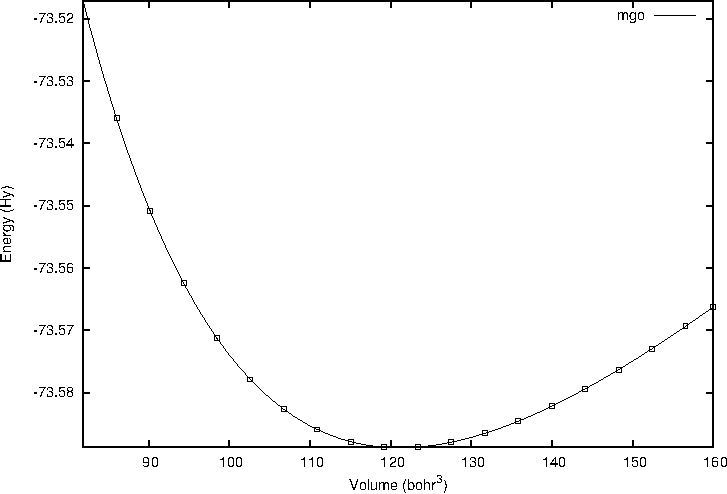
\includegraphics[scale=1.000000]{simple_efit.pdf}}

The points represent the original data and the solid line is a 12-th
degree polynomial in the Birch-Murnaghan strain. The fit is apparently
excellent.

Another important file is mgo.eos\_static, containing the static
properties derived from the E(V) curve (the first lines have been
wrapped, the rest have been trimmed for clarity):
%
\asciilist
\begin{lstlisting}
# Lines beginning with 'e' contain fit error estimation.
# Phase mgo
#    p(GPa)      E (Ha)     V(bohr^3)   V/V0    p_fit(GPa)\
               B(GPa)    Bp     Bpp(GPa-1)
    0.0000  -7.358887030E+01 121.1510 1.0000000    0.0000 \
             171.8631 4.1045942 -2.3291E-02
e   0.0000   0.000000000E+00   0.0016 0.0000130    0.0000 \
             0.0325 0.0089770  8.0853E-04
    5.0505  -7.356836447E+01 117.8343 0.9726230    5.0505 ...
e   5.0505   0.000000000E+00   0.0016 0.0000134    0.0000 ...
   10.1010  -7.354839133E+01 114.9271 0.9486271   10.1010 ...
e  10.1010   0.000000000E+00   0.0014 0.0000118    0.0000 ...
[...]
  141.4141  -7.312371446E+01  82.9321 0.6845349  141.4141 ...
e 141.4141   3.932099939E-06   0.0023 0.0000191    0.0000 ...
  146.4646  -7.310953178E+01  82.3100 0.6793997  146.4646 ...
e 146.4646   2.697398305E-06   0.0144 0.0001189    0.0000 ...
\end{lstlisting}

The calculated properties are the static energy, volume, compression,
bulk modulus and its pressure derivatives for a set of pressures. This
list of pressures can be controlled using the keyword \emph{pressure} (see
below). By default, gibbs2 calculated 100 pressure data points from 0
GPa to the maximum pressure allowed by the static energies, or 500
GPa. The lines beginning with an 'e' contain the error of the fit, as
estimated by the polynomial averaging technique.

The file mgo.eos contains the relation of the thermodynamic properties
calculated for the pressure and temperature conditions given in
input. For instance, in our example,
%
\asciilist
\begin{lstlisting}
# Phase mgo
# 01:p(GPa) 02:T(K) 03:V(bohr^3) 04:Estatic(Ha) 05:G(kJ/mol)
# 06:Gerr(kJ/mol) 07:p_sta(GPa) 08:p_th(GPa) 09:B(GPa) 10:U-Esta(kJ/mol)
# 11:Cv(J/molK) 12:F-Esta(kJ/mol) 13:S(J/molK) 14:ThetaD(K) 15:gamma
# 16:alpha(10^-5/K) 17:dp/dT(GPa/K) 18:Bs(GPa) 19:Cp(J/molK) 20:B_Tp
# 21:B_Tpp(GPa-1) 22:Fvib(kJ/mol) 23:Fel(kJ/mol) 24:Uvib(kJ/mol) 25:Uel(kJ/mol)
# 26:Svib(J/molK) 27:Sel(J/molK) 28:Cv_vib(J/molK) 29:Cv_el(J/molK)
#    p(GPa)      T(K)   V(bohr^3)    Estatic(Ha)        G(kJ/mol)    ...
      0.0000       0.00   123.0980  -7.358878E+01  -1.9319213537E+05 ...
      5.0505       0.00   119.6117  -7.358881E+01  -1.9313745955E+05 ...
     10.1010       0.00   116.5693  -7.358833E+01  -1.9308425053E+05 ...
       ...
    141.4141       0.00    83.6628  -7.352577E+01  -1.9195765650E+05 ...
    146.4646       0.00    83.0679  -7.352298E+01  -1.9192008494E+05 ...


      0.0000       6.57   123.0980  -7.358878E+01  -1.9319213537E+05 ...
       ...
    146.4646       6.57    83.0679  -7.352298E+01  -1.9192008494E+05 ...

       ...

      0.0000     650.12   125.8789  -7.358837E+01  -1.9321010456E+05 ...
       ...
    146.4646     650.12    83.3617  -7.352437E+01  -1.9192739359E+05 ...
\end{lstlisting}

The file is organized in sucessive blocks, one for each phase in the
input starting with the line '\# Phase' followed by the identifier of
the phase. After it, there is a header that specifies the
thermodynamic properties calculated and the field they occupy. The
data is organized in smaller blocks, one for each temperature, that
are separated by two blank lines (useful when using 'index' in
gnuplot, for example). These smaller blocks are composed of long
records each of them corresponding to the pressure and temperature
indicated in the first and second fields. The rest of the fields are
the calculated properties, as indicated in the header. As with the
pressure, the temperatures for which the properties are calculated can
be specified in the input, but in this simple example the default
list is used: 100 temperature data points from 0 to 1.5 times the
maximum Debye temperature.

The calculated properties are:
%
\begin{itemize}

\item %
\begin{description}
\item[{01:p(GPa)}] \leavevmode 
Pressure (given by the user).

\end{description}

\item %
\begin{description}
\item[{02:T(K)}] \leavevmode 
Temperature (given by the user).

\end{description}

\item %
\begin{description}
\item[{03:V(bohr\textasciicircum{}3)}] \leavevmode 
Equilibrium volume, V(p,T).

\end{description}

\item %
\begin{description}
\item[{04:Estatic(Ha)}] \leavevmode 
Static energy, interpolated at the equilibrium volume.

\end{description}

\item %
\begin{description}
\item[{05:G(kJ/mol)}] \leavevmode 
Gibbs free energy, G = E\_static + pV + F\_vib + F\_el + ... .

\end{description}

\item %
\begin{description}
\item[{06:Gerr(kJ/mol)}] \leavevmode 
The Helmholtz free energy contained can be calculated in two ways:
computing it directly using the equilibrium volume or by
interpolation from the fit. Gerr is the difference between both
approaches, and is usually negligible.

\end{description}

\item %
\begin{description}
\item[{07:p\_sta(GPa)}] \leavevmode 
Static pressure, -dE\_static/dV.

\end{description}

\item %
\begin{description}
\item[{08:p\_th(GPa)}] \leavevmode 
Thermal pressure, -(d(F-E\_static)/dV)\_T. Note that p = p\_sta + p\_th.

\end{description}

\item %
\begin{description}
\item[{09:B(GPa)}] \leavevmode 
Isothermal bulk modulus, B\_T = -V*(dp/dV)\_T = V*(d\textasciicircum{}2F/dV\textasciicircum{}2)\_T.

\end{description}

\item %
\begin{description}
\item[{10:U-Esta(kJ/mol)}] \leavevmode 
Non-static contribution to the internal energy: U\_vib + U\_el +...

\end{description}

\item %
\begin{description}
\item[{11:Cv(J/molK)}] \leavevmode 
Constant volume heat capacity, Cv = (dU/dT)\_V = Cv\_vib + Cv\_el +...

\end{description}

\item %
\begin{description}
\item[{12:F-Esta(kJ/mol)}] \leavevmode 
Non-static contribution to the Helmholtz free energy: F\_vib +
F\_el + ...

\end{description}

\item %
\begin{description}
\item[{13:S(J/molK)}] \leavevmode 
Entropy: S\_vib + S\_el + ...

\end{description}

\item %
\begin{description}
\item[{14:ThetaD(K)}] \leavevmode 
Debye temperature, only calculated for Debye-like models.

\end{description}

\item %
\begin{description}
\item[{15:gamma}] \leavevmode 
Gruneisen parameter, gamma = alpha * B\_T * V / C\_v =
V / C\_v * (dS/dV)\_T.

\end{description}

\item %
\begin{description}
\item[{16:alpha(10\textasciicircum{}-5/K)}] \leavevmode 
Volumetric thermal expansion coefficient, alpha = 1/V*(dV/dT)\_p =
gamma * C\_v / V / B\_T.

\end{description}

\item %
\begin{description}
\item[{17:dp/dT(GPa/K)}] \leavevmode 
(dp/dT)\_V = alpha * B\_T.

\end{description}

\item %
\begin{description}
\item[{18:Bs(GPa)}] \leavevmode 
Adiabatic bulk modulus B\_S = -V * (dp/dV)\_S = V*(d\textasciicircum{}2U/dV\textasciicircum{}2)\_S =
B\_T * (1 + alpha * gamma * T).

\end{description}

\item %
\begin{description}
\item[{19:Cp(J/molK)}] \leavevmode 
Constant pressure heat capacity, Cp = (dH/dT)\_p =
C\_v * (1+ alpha * gamma * T).

\end{description}

\item %
\begin{description}
\item[{20:B\_Tp}] \leavevmode 
Isothermal pressure derivative of the isothermal bulk modulus,
(dB\_T/dp)\_T.

\end{description}

\item %
\begin{description}
\item[{21:B\_Tpp(GPa-1)}] \leavevmode 
Isothermal second pressure derivative of the isothermal bulk
modulus, (d\textasciicircum{}2B\_T/dp\textasciicircum{}2)\_T.

\end{description}

\item %
\begin{description}
\item[{22:Fvib(kJ/mol)}] \leavevmode 
Vibrational contribution to the Helmholtz free energy.

\end{description}

\item %
\begin{description}
\item[{23:Fel(kJ/mol)}] \leavevmode 
Electronic contribution to the Helmholtz free energy (if no
electronic contribution model is used, 0).

\end{description}

\item %
\begin{description}
\item[{24:Uvib(kJ/mol)}] \leavevmode 
Vibrational contribution to the internal energy.

\end{description}

\item %
\begin{description}
\item[{25:Uel(kJ/mol)}] \leavevmode 
Electronic contribution to the internal energy.

\end{description}

\item %
\begin{description}
\item[{26:Svib(J/molK)}] \leavevmode 
Vibrational contribution to the entropy.

\end{description}

\item %
\begin{description}
\item[{27:Sel(J/molK)}] \leavevmode 
Electronic contribution to the entropy.

\end{description}

\item %
\begin{description}
\item[{28:Cv\_vib(J/molK)}] \leavevmode 
Vibrational contribution to the constant volume heat capacity.

\end{description}

\item %
\begin{description}
\item[{29:Cv\_el(J/molK)}] \leavevmode 
Electronic contribution to the constant volume heat capacity.

\end{description}

\end{itemize}

The two gnuplot scripts mgo\_all\_p.gnu and mgo\_all\_t.gnu are simple
ways of visualizing the information contained in the mgo.eos file. To
run them:
%
\asciilist
\begin{lstlisting}
gnuplot mgo_all_p.gnu
gnuplot mgo_all_t.gnu
\end{lstlisting}

This creates a good number of pdf files called mgo\_p\_xx.pdf
and mgo\_t\_xx.pdf. The mgo\_p\_xx.pdf file represents the isotherms of
the xx property versus pressure, where xx is one of the numeric labels
above. The mgo\_t\_xx.pdf represent the temperature depenedence of the
xx property at p = 0 GPa. For our example, mgo\_p\_03.pdf are the
calculated V(p) isotherms and mgo\_t\_03.pdf is a plot representing
thermal expansion at zero pressure:

\noindent\makebox[\textwidth][c]{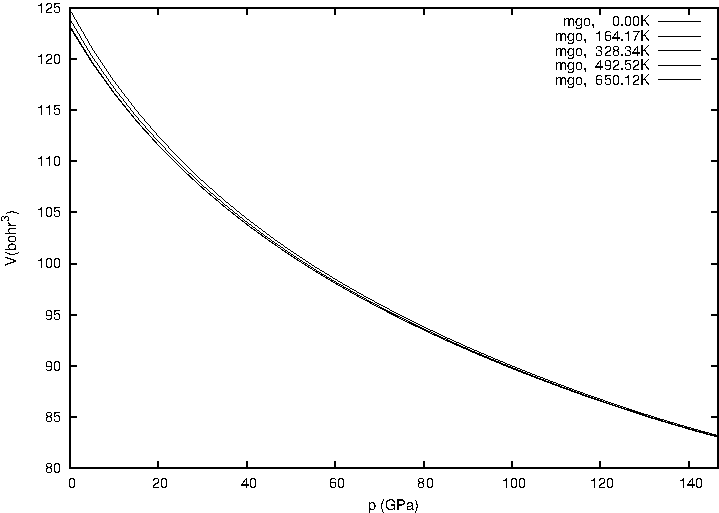
\includegraphics[scale=1.000000]{simple_mgo_p_03.pdf}}

\noindent\makebox[\textwidth][c]{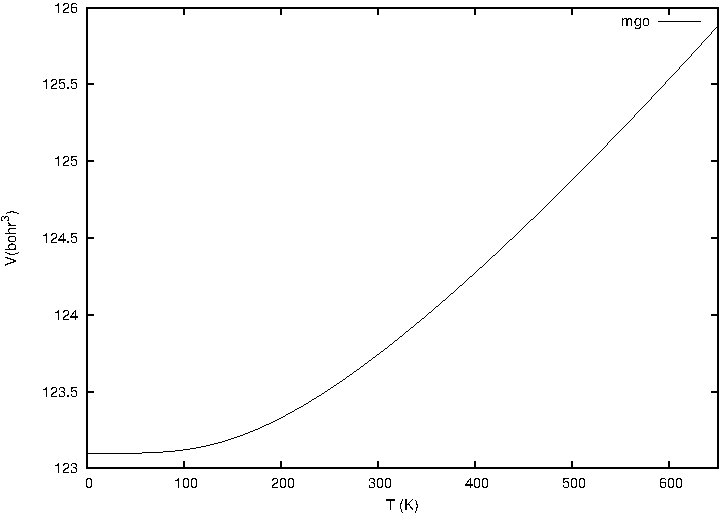
\includegraphics[scale=1.000000]{simple_mgo_t_03.pdf}}

Similarly, mgo\_p\_09.pdf contains several curves representing the
pressure dependence of the bulk modulus at the computed temperatures
and mgo\_t\_09.pdf is a plot of B\_T(T) at 0 pressure:

\noindent\makebox[\textwidth][c]{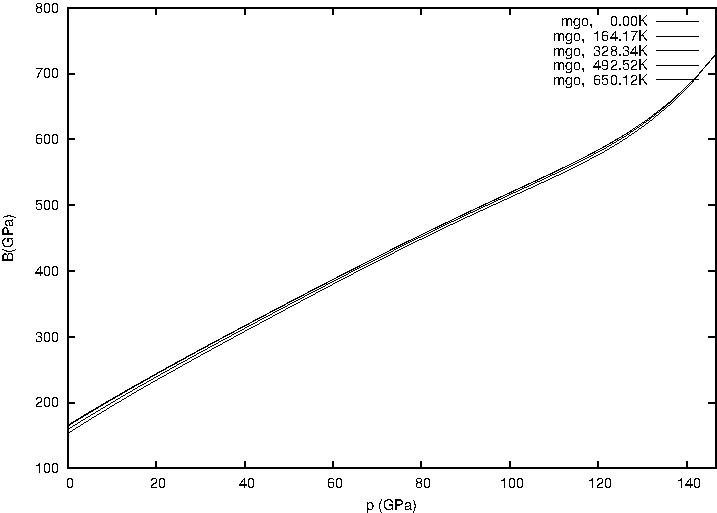
\includegraphics[scale=1.000000]{simple_mgo_p_09.pdf}}

\noindent\makebox[\textwidth][c]{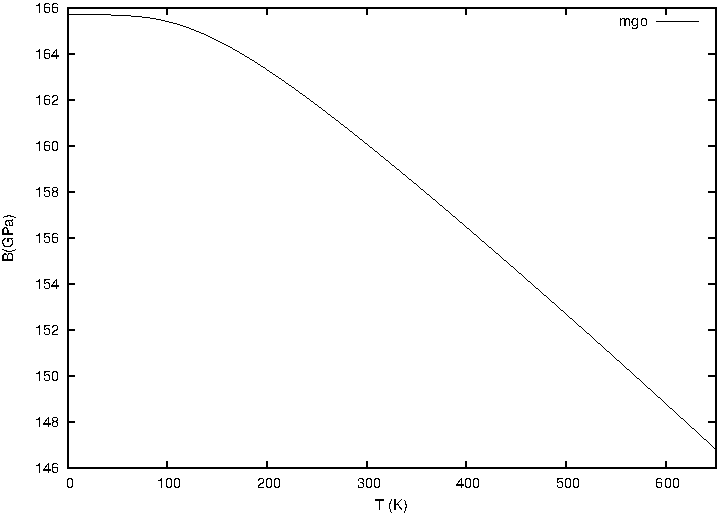
\includegraphics[scale=1.000000]{simple_mgo_t_09.pdf}}

The standard output file generated by gibbs2, mgo.out, contains useful
information and a detailed relation of the auxiliary output files. It
is structured in blocks denoted by a header that starts with an
asterisk. For instance, the first block (Input) contains information
about the input values of some general variables, and it is
self-explanatory:
%
\asciilist
\begin{lstlisting}
* Input
  Title:
  Output file (lu= 2): stdout
  Units: output is in atomic units, except where noted.
  Number of atoms per formula:   2
  Molecular mass (amu):       40.30440000
  ...
\end{lstlisting}

Following this section, the pressure range is displayed. We have
used the default pressures, so gibbs2 automatically sets this list to
100 points from 0 to the maximum pressure attainable with the input
data, p\_max. This p\_max is calculated as the slope at the point of the
volume grid with smallest volume: any pressure higher than p\_max would
preclude the appearance of the minimum of the static enthalpy on the
volume grid:
%
\asciilist
\begin{lstlisting}
* Pressure range examined
  Min_phases{p_max} (GPa):      118.529
  Pressure range (GPa):        0.000 ->      500.000
  Number of p points:    100
  New pressure range (GPa):        0.000 ->      146.465
  New number of p points:     30
\end{lstlisting}

Next, the information about the phases is presented, including static
equilibrium properties, statistical measures about the quality of the
static fit, and the static equation of state, much like in the
mgo.eos\_static file:
%
\asciilist
\begin{lstlisting}
* Phase information after initial setup
+ Phase  1 (mgo)
  Number of volume points:   20
  p(V) input data? F
  Pressure range (GPa):      -27.115 ->      118.529
  Number of interpolated fields :    0
  Input units:
    Volume : bohr^3
  ...
  Temperature model: Debye, Td from static B(V).
  All data points are ACTIVE for dynamic calculations

  Fit to static E(V) data:
# Copy in file : mgo.eos_static
# Lines beginning with 'e' contain fit error estimation.
#    p(GPa)          E (Ha)     V(bohr^3)      V/V0   p_fit(GPa)   B(GPa)         Bp      Bpp(GPa-1)
      0.0000  -7.358887030E+01   121.1510  1.0000000     0.0000   171.8631    4.1045942  -2.3291E-02
e     0.0000   0.000000000E+00     0.0016  0.0000130     0.0000     0.0325    0.0089770   8.0853E-04
  ...
\end{lstlisting}

The static energy plots are calculated next, and the Debye
temperatures are computed. The default thermal model is the Debye
model in the Slater formulation: the Debye temperatures, Td(V) are
computed from the static bulk moduli B(V), and the Poisson ratio is
assumed to be volume independent, and equal to 1/4. This information
is presented in the output:
%
\asciilist
\begin{lstlisting}
* Computed Debye temperatures from static data
+ Phase mgo
# ThetaD at static eq. volume:     836.45
# V(bohr^3)  Tdebye(K)   Tdebye_slater(K)
    81.8884    1575.07    1575.07
    86.0359    1460.24    1460.24
 90.1834    1364.07    1364.07
 94.3309    1274.15    1274.15
...
160.0000     433.41     433.41
\end{lstlisting}

The minimum of Td(V) is usually found at the largest volume. This
Td\_min is used to set the default temperature datasets used in the
dynamic calculation:
%
\asciilist
\begin{lstlisting}
* Temperature range examined
  Min_{DebyeT} (K):      433.415
  Temperature range (K):        0.000 ->      650.122
  Number of T points:    100
\end{lstlisting}

Once the static calculation is over, gibbs2 loops over temperatures
and pressures and calculates the thermodynamic properties for each pT
point, and writes the results to the eos file:
%
\asciilist
\begin{lstlisting}
* Calculated temperature effects
  Writing file : mgo.eos
\end{lstlisting}

A final note: it is usually convenient to keep the gibbs2 input file
separated from the actual phase data. The keywords \emph{file} and \emph{using}
(or \emph{u} for short) can be used in \emph{phase} to read an external file
containing the volume and energy data. For instance, mgo.ing could be:
%
\gibbslist
\begin{lstlisting}
mm 40.3044
vfree 2
phase mgo file mgo.dat u 1:3
\end{lstlisting}

and the E(V) data would be read from the fields 1 and 3.


\subsection{4.2~~~Fitting equations of state%
  \label{fitting-equations-of-state}%
}

We continue with a slightly more complex example. The following input
file reads an external file (c.dat) containing the energy-volume curve
of diamond (PBE), and applies several different fits to the
data, using the Debye-Gruneisen tempearture model. Each equation of
state examined corresponds to one \textbf{phase} keyword: the dataset is
always the same, but the model representation given by the equation of
state used to fit the data changes.

The input file is:
%
\gibbslist
\begin{lstlisting}
set notrans
mm 24.0214
vfree 2
pressure 0
temperature 0 10 3000

phase BM3 file c.dat tmodel debye_gruneisen dm \
          units energy ry \
          fit strain bm 3
phase BM4 file c.dat tmodel debye_gruneisen dm \
          units energy ry \
          fit strain bm 4
phase PT3 file c.dat tmodel debye_gruneisen dm \
          units energy ry \
          fit strain pt 3
phase PT4 file c.dat tmodel debye_gruneisen dm \
          units energy ry \
          fit strain pt 4
phase Vinet file c.dat tmodel debye_gruneisen dm \
          units energy ry \
          fit vinet
end
\end{lstlisting}

and the data file (c.dat) is:
%
\asciilist
\begin{lstlisting}
40.000000000000000 -22.107087940000000
41.666666666666664 -22.204061660000001
...
\end{lstlisting}

Note the first lines in the input are preceded by '\#': this means
these lines are comments, and therefore are ignored by gibbs2. Note
also the backslashes that continue \textbf{phase} lines. The \textbf{notrans}
option is activated with a \textbf{set} keyword. \textbf{set} keywords modify
the global behavior of gibbs2: an exhaustive relation of these options
can be found in the reference section of this manual. The \textbf{notrans}
option deactivates the calculation of the phase diagram (transition
pressures, most stable phase,...). It is clear that in this case it is
not meaningful. The \textbf{mm} and \textbf{vfree} keywords are the same as in
the previous example: the primitive cell of diamond contains 2 atoms,
and the molecular weight is 2 times the mass of a carbon atom. The
thermodynamic properties are calculated only at null pressure, and in
a temperature grid spanning from 0 to 3000 K in steps of 10 K.

Five phases are defined, each of them using the same dataset
(contained in the file c.dat), which is interpreted to be a list of
volumes (in bohr\textasciicircum{}3, the default) and energies in Ry, because of the
\textbf{units} keyword. All of them use the same temperature model
(Debye-Gruneisen with Dugdale-McDonald gamma) and different equations
of state. The equations of state used are Birch-Murnaghan (3rd and 4th
order), Poirier-Tarantola (3rd and 4th order) and Vinet. All of them
carry out linear fits of the energy versus some strain except in the
case of Vinet. This and other technical details of the fit are treated
below, in the reference for the \textbf{fit} keyword.

The structure of the output is more or less the same as in the
previous example, but each phase receives its own block inside each of
the sections. Plotting the temperature dependence of the properties
with:
%
\asciilist
\begin{lstlisting}
gnuplot c_all_t.gnu
\end{lstlisting}

yields, for instance, a B\_S(T) plot like the following:

\noindent\makebox[\textwidth][c]{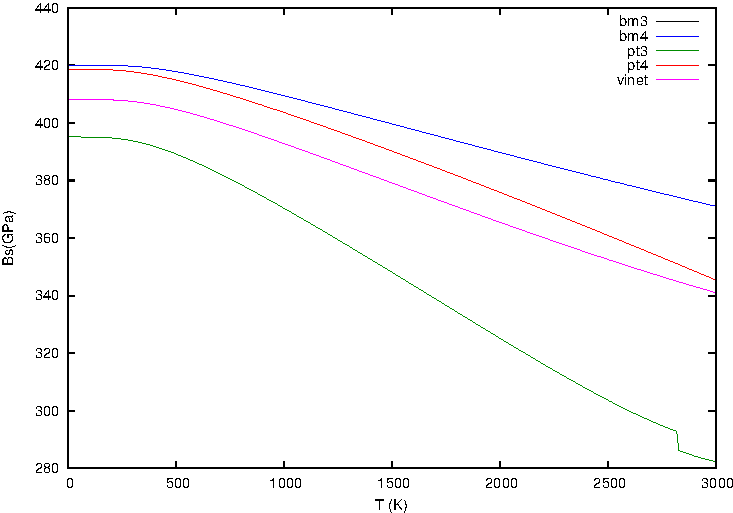
\includegraphics[scale=1.000000]{fits_c_t_18.pdf}}

Judging from this picture, it is clear that choosing a good equation
of state is very important. At 2000 K, the range spanned by different
equations of state is as large as 80 GPa. The recommended procedure in
gibbs2 is using an average of polynomials in a given strain (for
instance, a BM strain). This method, in addition, provides a good
estimation of the quality of the fit by means of error bars of the
calculated properties. It is interesting to note that, in spite of the
dramatic differences between EOS in the B\_S(T) curve, the
energy-volume curve is superbly represented by \emph{all} the EOS used:
%
\asciilist
\begin{lstlisting}
gnuplot c_efit.pdf
\end{lstlisting}

\noindent\makebox[\textwidth][c]{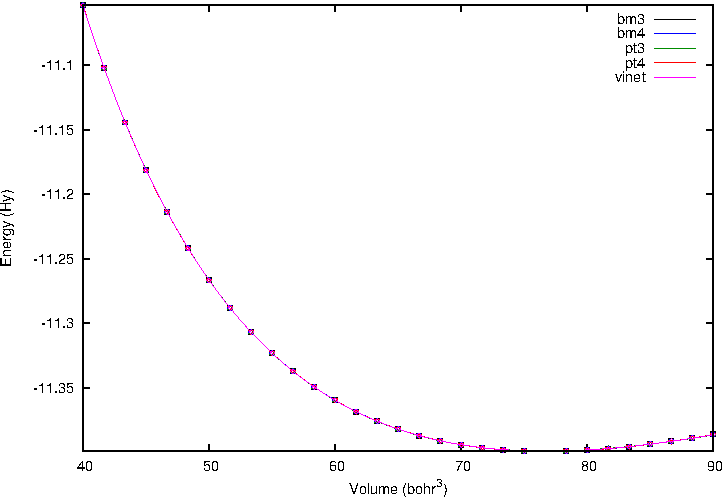
\includegraphics[scale=1.000000]{fits_c_efit.pdf}}

Unfortunately, this plot is too often a criterion of the quality of a
fit in the literature.

It is important to note that gibbs2 is not designed for
extrapolation. This means that the thermodynamic properties are never
calculated on equilibrium volumes outside of the input volume grid.

A final note: in cases when the input dataset contains few points, the
default maximum strain polynomial degree (mpar = 12) may be inadequate
and cause an overfitting problem. In such cases, it is wise to use the
\emph{set mpar} keyword (see below) to set this parameter to a lower
value.


\subsection{4.3~~~Temperature models%
  \label{temperature-models}%
}

Gibbs2 implements several models for the inclusion of temperature
effects to the results of an ab initio calculation. The models
provided cover a range of complexity (and accuracy), with the Debye
model in Slater's implementation being the most simple and the full
quasiharmonic approximation being the most complex. Likewise, more
complex temperature models require that the user provides larger
quantities of data: for instance, the Debye model requires only the
input of the static E(V) curve (and optionally the experimental
Poisson ratio), while the QHA model requires the phonon spectrum
calculated at each grid volume. The Debye-Gruneisen model is an
improvement upon the simple Debye model. The quasiharmonicity
introduced by assuming that the Poisson ratio does not change with
volume is corrected by assuming an approximate Grüneisen gamma, such
as Dugdale-McDonald's formula. With it, it is possible to get a more
realistic evolution of the Debye temperature parameter than in the
original Slater's model.

Also, in molecular crystals, it is usually necessary to account for
the (probably many) optic branches of the spectrum. To that end, the
Debye-Einstein model reads the optic frequencies at gamma and builds a
phonon spectrum using a Debye model for the acoustic part, and a sum
of Dirac deltas for the optic part, centered around the Gamma
frequencies. The temperature models are explained in full in the
reference section and in the companion articles.

Let us illustrate the use of the various models with a simple
example. The following input compares different models on the B1 phase
of MgO (calculated with PP+PW, PBE xc functional).
%
\gibbslist
\begin{lstlisting}
set notrans
mm 40.3044
vfree 2
pressure 0 1 250
temperature -1

phase debye file ../dat/mgo_pbe/mgo.res tmodel debye \
                units energy ry freq cm-1 \
                prefix ../dat/mgo_pbe/
phase debgrun file ../dat/mgo_pbe/mgo.res tmodel debye_gruneisen dm \
                units energy ry freq cm-1 \
                prefix ../dat/mgo_pbe/
phase debeins file ../dat/mgo_pbe/mgo.res tmodel debye_einstein \
                units energy ry freq cm-1 \
                prefix ../dat/mgo_pbe/
freqg0 debeins
  402.9580 402.9580 701.1656
endfreqg0
phase qha file ../dat/mgo_pbe/mgo.res tmodel qha \
                units energy ry freq cm-1 \
                prefix ../dat/mgo_pbe/
end
\end{lstlisting}

In this case, we calculate the pressure dependence of the
thermodynamic properties with pressure (up to 250 GPa) at room
temperature (\textbf{temperature} -1). Each model corresponds to a
\textbf{phase} keyword, all of them using the same dataset and even the
same input file, consisting of:
%
\asciilist
\begin{lstlisting}
40.000000000000000 -145.125645270000007 001_/001_.phdos
40.700434586218826 -145.213514589999988 002_/002_.phdos
...
160.000000000000000 -147.254963110000006 129/129.phdos
\end{lstlisting}

Depending on the model, some or all of these fields are read. In the
Debye model, the fields 1 and 2 (volume and energy) are read and the
third field that points to the phonon DOS is ignored. Note that the
files containing the phonon DOS are located in a subdirectory 'xxx/'
relative to the directory of the input data file, which in turn is
located in '../dat/mgo\_pbe/' relative to the gibbs2 input file. To
make gibbs2 find the phonon DOS files, it is necessary to include a
'prefix' keyword, whose argument is preprended to the phonon DOS file
names. For instance, for the first file, '%
\raisebox{1em}{\hypertarget{id14}{}}\hyperlink{id13}{\textbf{\color{red}001\_}}/%
\raisebox{1em}{\hypertarget{id16}{}}\hyperlink{id15}{\textbf{\color{red}001\_}}.phdos', prepending
the prefix '../dat/mgo\_pbe/' yields the file
'../dat/mgo\_pbe/%
\raisebox{1em}{\hypertarget{id18}{}}\hyperlink{id17}{\textbf{\color{red}001\_}}/%
\raisebox{1em}{\hypertarget{id20}{}}\hyperlink{id19}{\textbf{\color{red}001\_}}.phdos', which is the correct path relative
to the gibbs2 input file. It is also possible to use absolute path
prefixes.

The Debye-Einstein model requires the frequencies at the Gamma point
for the equilibrium geometry, which are included using the \textbf{freqg0}
keyword, which associates its input to a phase using its string or
integer label (in this case, 'debeins' or 3). MgO has 3 optic
branches, so there are 3 frequencies at Gamma to be input, in cm\textasciicircum{}-1,
as indicated in the \textbf{units} section of the phase.

A preview of the results can be plotted running gnuplot on the
'all\_p.gnu' script. For instance, the result for the thermal pressure
is:

\noindent\makebox[\textwidth][c]{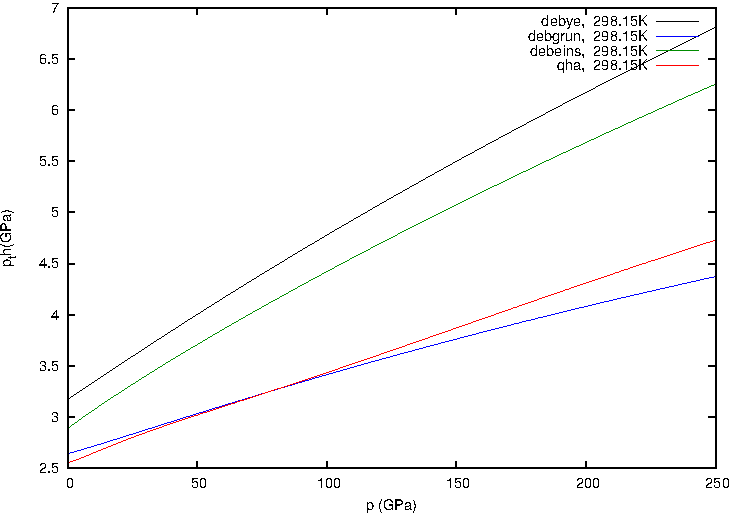
\includegraphics[scale=1.000000]{tmodels_mgo_pth.pdf}}

As the MgO is a closely packed material with not many optic branches
the result of the Debye models is quite reasonable, provided a good
evolution of the Debye temperature with pressure is used. Thus,
Debye-Gruneisen results are very close to QHA while the simple Debye
model and Debye-Einstein are farther from the correct quasiharmonic
result. The inclusion of the frequencies at Gamma shifts the thermal
pressure towards the QHA result with a small step.


\subsection{4.4~~~Empirical corrections of the energy%
  \label{empirical-corrections-of-the-energy}%
}

The thermodynamic properties resulting from a density functional
calculation most of the time depend dramatically on the
exchange-correlation density functional employed, which is the main
source of error contained in their calculation provided a good
temperature model is used. In order to correct these discrepancies,
empirical energy corrections (EEC) have been proposed.

The EEC are corrections on the static energy curve that force the
model to meet experimental data. In the current implementation one
datum (the experimental equilibrium volume at ambient conditions) or
maybe two (the experimental bulk modulus at ambient conditions) are
used. Several EECs have been implemented, which are described in full
in the reference section and in xxxx. These are the 'pshift'
correction (shift the energy with a constant pressure), the 'apbaf'
(adding a constant times 1/V) and the 'bpscal' (using the observation
that p/B0 versus v/v0 is similar for all functionals and experimental
data).

In the next example, the three EECs and the unscaled results are
calculated for the diamond:
%
\asciilist
\begin{lstlisting}
# Diamond
# Bulk modulus: 446 (Occelli2004)
# V0 : 3.4170 cm3/mol (/ 6.02214179e23 * 2 * 1e24 / .52917720859^3) =
# = 76.58092 (Occelli2004)
set notrans
mm 24.0214
vfree 2
pressure 0
temperature 0 10 3000

phase LDA:uncorr file ../dat/c_lda/c.res tmodel qha \
                 units energy ry freq cm-1 \
                 prefix ../dat/c_lda/
phase PBE:uncorr file ../dat/c_pbe/c.res tmodel qha \
                 units energy ry freq cm-1 \
                 prefix ../dat/c_pbe/
phase LDA:pshift file ../dat/c_lda/c.res tmodel qha \
                 units energy ry freq cm-1 \
                 prefix ../dat/c_lda/ \
                 eec pshift 76.58092
phase PBE:pshift file ../dat/c_pbe/c.res tmodel qha \
                 units energy ry freq cm-1 \
                 prefix ../dat/c_pbe/ \
                 eec pshift 76.58092
phase LDA:apbaf  file ../dat/c_lda/c.res tmodel qha \
                 units energy ry freq cm-1 \
                 prefix ../dat/c_lda/ \
                 eec apbaf 76.58092
phase PBE:apbaf  file ../dat/c_pbe/c.res tmodel qha \
                 units energy ry freq cm-1 \
                 prefix ../dat/c_pbe/ \
                 eec apbaf 76.58092
phase LDA:bpscal file ../dat/c_lda/c.res tmodel qha \
                 units energy ry freq cm-1 \
                 prefix ../dat/c_lda/ \
                 eec bpscal 76.58092 446
phase PBE:bpscal file ../dat/c_pbe/c.res tmodel qha \
                 units energy ry freq cm-1 \
                 prefix ../dat/c_pbe/ \
                 eec bpscal 76.58092 446
end
\end{lstlisting}

We have used the full QHA model for temperature effects and applied
the correction using the experimental volume of the primitive cell
(76.58092 bohr\textasciicircum{}3) and the experimental bulk modulus (446) at room
temperature. Running the '\_all\_t.gnu' script file with gnuplot gives:

\noindent\makebox[\textwidth][c]{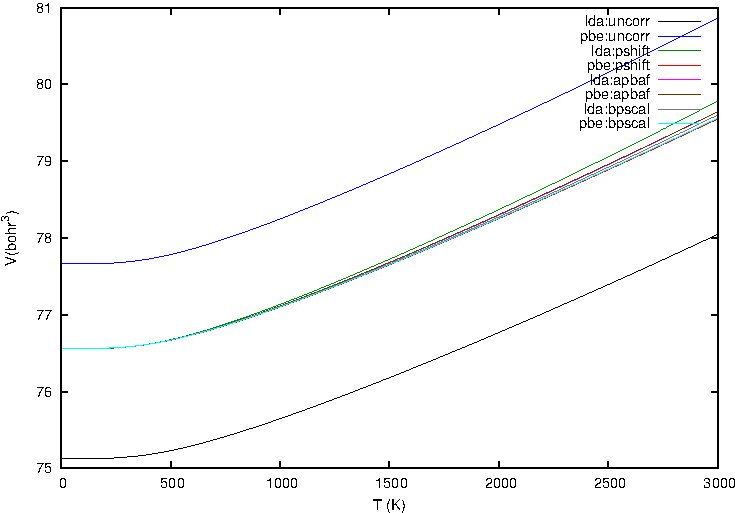
\includegraphics[scale=1.000000]{eec_t_v.pdf}}

\noindent\makebox[\textwidth][c]{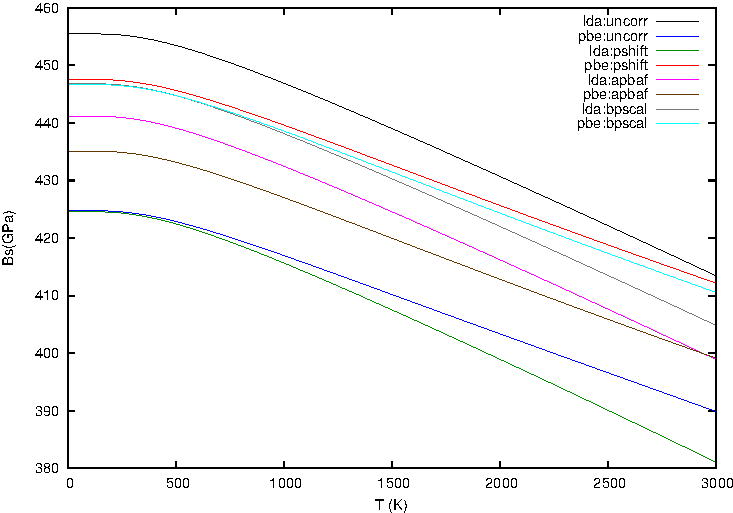
\includegraphics[scale=1.000000]{eec_t_bs.pdf}}

The first graph is a plot of the calculated volume with
temperature. Observe the enormous gap between uncorrected LDA and PBE
results, which is reduced to a very close match by energy
corrections (and which agree very well with experimental data). All
the EECs seem to perform very well for the calculation of V(T), with
pshift perhaps being the farthest from the others. The differences in
the volume representation are widened when one turns to the
calculation of the adiabatic bulk modulus. Again, there is an enormous
gap in the uncorrected results. As the bulk modulus is a property that
depends mostly on the derivatives of the energy, and not energy
itself, the EECs peformance varies according to their definition, but
all of them seem to improve the result. The best EEC seems to be
'bpscal' which corrects the data to enforce the experimental bulk
modulus. The LDA and PBE results corrected with bpscal match closely
for lower temperatures and deviate at higher temperatures. The
difference between them, though, is still far lower than for the
uncorrected gap.


\subsection{4.5~~~The electronic contribution to the free energy%
  \label{the-electronic-contribution-to-the-free-energy}%
}

In addition to the vibrational, metals possess electronic degrees of
freedom that contribute to the free energy and the heat
capacity. These arise from their band structure: the electrons are
free to roam the metal because there are empty states at arbitrarily
small energies above the Fermi level. Usually, this contribution to
the free energy is negligible compared to the vibrational. However,
due to its simplicity, gibbs2 provides a means for including it using
two different models: the Sommerfeld model of free and independent
electrons (\textbf{sommerfeld}) and a model that reads the coefficients of
a polynomial fitted to results of finite temperature DFT calculations
(see Mermin, 1965).

We can illustrate this with the following simple example, where we
calculate the properties of fcc aluminium:
%
\gibbslist
\begin{lstlisting}
# Aluminium
set notrans
mm 26.981538
vfree 1
pressure 0
temperature -1
volume input

phase Al:free file ../dat/al_lda/al.res tmodel qha phfield 12 \
         units energy ry freq cm-1 \
         prefix ../dat/al_lda/ eec bpscal 112.04 72.7 \
         elec sommerfeld free nelec 3
phase Al:somm_nef file ../dat/al_lda/al.res tmodel qha phfield 12 \
         units energy ry freq cm-1 edos ev \
         prefix ../dat/al_lda/ eec bpscal 112.04 72.7 \
         elec sommerfeld nelec 3
phase Al:pol4 file ../dat/al_lda/al.res tmodel qha phfield 12 \
         units energy ry freq cm-1 \
         prefix ../dat/al_lda/ eec bpscal 112.04 72.7 \
         elec pol4 4
end
\end{lstlisting}

The primitive cell of fcc aluminium contains one atom, with molecular
weight 26.981538 amu. The pressure list is composed only of the zero
pressure point and the temperature is room temperature. It is possible
direct gibbs2 to calculate the properties at given temperatures on a
list of volumes instead of pressures with the \textbf{volume} keyword. The
\textbf{volume input} order instructs gibbs2 to calculate the properties at
the input grid of volumes.

Three phases are included in the input, each representing a different
electronic model. The first phase corresponds to the free electron
model, which is activated using the \textbf{elec sommerfeld free}
order. The model requires the number of conduction electrons per
primitive cell, 3 in this case. The energy is corrected to yield the
experimental volume (112.04 bohr\textasciicircum{}3) and bulk modulus (72.7 GPa) of
aluminium with an EEC as described above, which can be used with
different temperature and electronic models. The second phase
corresponds to the free electron model but where the population at the
Fermi level, N(Ef), is read from the input file. This is achieved by
omitting the \textbf{free} keyword. In the third phase, the coefficients of
the fourth degree polynomial that fits F\_el (the electronic Helmholtz
free energy) and -T*S\_el with respect to temperature are read. This
option requires the usage of an external fitting script to find the
coefficients.

The input datafile is always the same (al.res), and its structure is
(the backslashes are not contained in the original input file, the
lines have been wrapped for clarity):
%
\asciilist
\begin{lstlisting}
35.200000000000003 -11.447724709999999  0.203700 2.0620541311e-09 \
-1.8439425798e-10  7.4740480714e-15  -5.5458673605e-18 \
-9.2793212377e-10 -3.5154688019e-10  -9.1949143703e-15 \
-4.2538048412e-18  012_/012_.phdos
...
\end{lstlisting}

As always, the first field is the primitive cell volume and the second
is the energy. Then, N(Ef) in 1/eV (see \textbf{units edos} in the ing
file above) and the 8 polynomial coefficients. The first 4
coefficients (fields 4 to 7) fit F\_el with respect to T (T coefficient
is field 4, T\textasciicircum{}2 is field 5,... there is no independent term because
F\_el(0) = 0). The next 4 coefficients (fields 8 to 11) fit -T*S\_el to
temperature. The units of both F\_\{el\} and -T*S\_\{el\} are the units set
by the \textbf{units energy} keyword, that is, Ry. The last field points to
the phonon density of states file for that volume.

The ordering of the fields must be treated carefully. By default, the
interpretation sequence is: volume, energy, Debye temperature, N(Ef),
coefficients of F\_el, coefficients of -T*S\_el and phonon file (DOS or
frequencies). Depending on the phase, some of these fields are read
and some are not. This order is, however, not compulsory, and the
order of each of the fields can be modified by the appropriate
keyword. In the first phase, the free electron model and QHA are
used. The free elctron model does not need any of the above variables,
but QHA does require the vibrational input file. Because the default
field for phdos1.s is 3 (only volume and energy are read, and come
before the phDOS field), it is necessary to indicate to gibbs2 that
the file is actually located in field 12 in the input file. This is
achieved using the \textbf{phfield} keyword after \textbf{qha}. The same applies
to the other two phases.

In the second phase, the free electron model with N(Ef) input is
used. The field from which the N(Ef) is read can be changed using an
integer right after the \textbf{sommerfeld} keyword. If no integer is
found, then the default field is used. In the al.res input file, N(Ef)
appears on the third field, right after the energy. As the Debye
temperature is not read in QHA, 3 is the default field for N(Ef), and
it is not necessary to write explicitly the field where N(Ef) lives.

In the third phase, the 8 polynomial coefficients and the phDOS file
are read. The default field for the first polynomial coefficient is 3,
but the position it occupies in the file is 4, so it is necessary to
write it explicitly in the input line, after \textbf{pol4}. Note that the 8
coefficients must always appear in sequence, with the correct order.

The following plot represents the results of the above input:

\noindent\makebox[\textwidth][c]{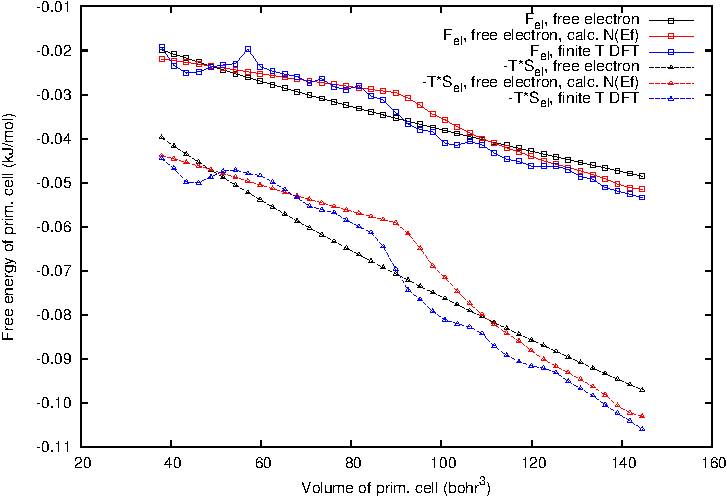
\includegraphics[scale=1.000000]{elec_v_f.pdf}}

It represents the electronic Helmholtz free energy (the upper bunch of
curves) and -T*S\_el against the input volume grid. Al is the prototype
of a free electron metal, which is clearly confirmed by the
aparametric free electron model rendering free energies extremely
close to those calculated by ab initio programs. Note the noise in the
calculated F\_el and TS\_el and even in the Sommerfeld model using the
external N(Ef). One kelvin is more or less pi microHartree, so it is
clear that the energy correction a moderate temperature (say, 500 K)
has on the static energy is quite small. Therefore, the accuracy of
this correction is extremely dependent on the calculation parameters
and, in particular, on the k-point grid. The results shown above are
calculated using a 52x52x52 Monkhorst-Pack grid. A final note: the
magnitude of F\_el is small (some \%) compared to F\_vib, so the
thermodynamic properties (equilibrium volumes, bulk moduli, etc.) are
barely affected, except at extremely low temperatures.


\subsection{4.6~~~Phase transitions%
  \label{phase-transitions}%
}

Contrarily to the old gibbs, gibbs2 can actually calculate stability
diagrams and transition pressures between different phases of the same
solid by calculating the Gibbs free energy for each of them and then
determining the most stable phase in the input at given pressure and
temperature conditions.

In the next example, we have calculated the transition pressures with
temperature of MgO, from the very stable B1 -> B2 phase. It is clear
from the literature that this transition occurs around 500 GPa, but
it has not been experimentally observed yet (jan. 2011).

An important note: when comparing phases with different number of
atoms in the cell it is necessary to scale the extensive quantities
given in input (volume, energy,...). See the \textbf{vfree} and \textbf{z}
keywords for further information.

The input file for the MgO B1 -> B2 is:
%
\asciilist
\begin{lstlisting}
mm 40.3044
vfree 2
pressure 0 25 600
temperature 0 20 1000

phase B1 file ../dat/mgo_pbe/mgo.res tmodel qha \
                 units energy ry freq cm-1 \
                 prefix ../dat/mgo_pbe/ \
                 eec bpscal 126.025 161.3
phase B2 file ../dat/mgob2_pbe/mgob2.res tmodel qha \
                 units energy ry freq cm-1 \
                 prefix ../dat/mgob2_pbe/ \
                 eec use 1
end
\end{lstlisting}

This time, each \textbf{phase} keyword corresponds to a physical phase, and
the two data files are different. Note that the energy correction is
applied as usual to the first phase, B1, which is the stable phase at
ambient conditions. There is absolutely no experimental information
about the B2 phase, so we opt here to use the same correction
coefficients as in the B1 phase (number 1), with \textbf{eec use 1}.

The gibbs2 output contains the static transition pressures:
%
\asciilist
\begin{lstlisting}
* Static transition pressures (linear interpolation)
#        Pressure range (GPa)      Stable phase
        0.0000 -->     503.1471          b1
      503.1471 -->     600.0000          b2
\end{lstlisting}

The static transition pressure is 503.1 GPa, more or less the same
result as other authors found for this transition. In addition, gibbs2
generates a number of auxiliary files:
%
\begin{itemize}

\item 06\_phases\_dH.gnu, 06\_phases\_dH.aux : this files generate a plot of
the difference in static enthalpy between all the phases and the
first phase in the input. In this case, the plot is:

\end{itemize}
%
\begin{itemize}

\item 06\_phases.tpstab : a file containing the identity, Gibbs free
energy, volume and adiabatic bulk modulus of the stable phase at
each pressuer and temperature data point.

\item 06\_phases.dgtp : difference in Gibbs free energy between all the
calculated phases and the first, for all the temperature and
pressure data points.

\item 06\_phases.ptrans, 06\_phases\_ptrans.gnu : a plot of the evolution of
the transition pressure with temperature. A slight modification of
the gnu file yields:

\end{itemize}
%
\asciilist
\begin{lstlisting}
 #      T(K)                 b1              b2
        0.0000        0.0000 ->     492.1215 ->     600.0000
       20.0000        0.0000 ->     492.1215 ->     600.0000
       ...

Each '->' symbol corresponds to a stability domain, *not* a
transition. For instance, at 20 K, the B1 phase is stable from 0 to
492.1 GPa. The B2 phase is stable from the latter pressure to 600
GPa at least. 600 GPa is the highest pressure explored in the input.
\end{lstlisting}


\section{5~~~Keyword reference%
  \label{keyword-reference}%
}


\subsection{5.1~~~General purpose keywords%
  \label{general-purpose-keywords}%
}

A full list of the gibbs2 input syntax follows. Integer, real and
string variables are denoted by i, r and s suffixes
respectively. Optional arguments are enclosed in
brackets. Alternatives are grouped by curly braces and separated using
a bar (|).
%
\begin{itemize}

\item \textbf{\# This is a commment}
%
\begin{quote}

Comment lines begin with a \# character. Lines are continued with a
backslash () character

\end{quote}

\item \textbf{title title.s}
%
\begin{quote}

The title of the run.

\end{quote}

\item \textbf{nat nat.i}, \textbf{vfree nat.i}
%
\begin{quote}

Number of atoms per (primitive) unit cell or per unit formula (both
keywords are equivalent). Any multiple of the basic unit formula
can be used, provided some conditions are met. These conditions
are:
%
\begin{itemize}

\item In the \textbf{static} temperature model, \textbf{nat.i} is not used
whatsoever, so this keyword can be omitted. However, volumes and
energies must be consistent with each other.

\item In \textbf{debye} and \textbf{debye\_gruneisen}, nat.i and \textbf{mm} must
refer to the same basic unit of repetition. In addition,
nat.i times the \textbf{Z} of each phase (see the PHASE keyword
below) must be the number of atoms for which energies and volumes
are calculated. If the model is \textbf{debye\_input}, then the Debye
temperatures must be normalized to \textbf{nat.i} atoms.

\item In \textbf{debye\_einstein}, the same as in \textbf{debye} applies. The
number of frequencies read is 3 x \textbf{nat.i} x \textbf{Z} - 3, where
\textbf{Z} depends on the phase.

\item In \textbf{qha}, the same as in \textbf{debye} applies. Additionally, the
phonon DOS must be normalized to 3 x \textbf{nat.i} x \textbf{Z}.

\item In \textbf{qha\_espresso}, the same as in \textbf{debye} applies. The number
of frequencies read is 3 x \textbf{nat.i} x \textbf{Z} for each reciprocal
space point.

\end{itemize}

Note that, with indenpendence of the temperature model used, the
phonon density of states are renormalized to \textbf{nat.i} so the
extensive quantities in the output are per \textbf{nat.i} atoms,
regardless of the \textbf{Z} of each phase. This allows free energy
comparisons.

To simplify, unless there is a good reason (e.g. two different
phases with different number of non-equivalent atoms and hence
frequencies per k-point), it is easier to input quantities per
primitive cell.

\end{quote}

\item \textbf{mm mm.r}
%
\begin{quote}

Mass (amu) per unit containing nat.i (defined using \textbf{vfree})
atoms.

\end{quote}

\item \textbf{nelectrons nelec.i}
%
\begin{quote}

Total number of electrons in the primitive unit cell. This value is
used only if any of the phases is fit using Holzapfel's AP2. The
value of this variable implies nothing to the value of the
\textbf{nelec} keyword in the \textbf{phase} keyword.

\end{quote}

\item \textbf{einf einf.r}
%
\begin{quote}

Energy at V=Inf. Used only for the scaling of the extensive
energetic properties (default 0).

\end{quote}

\item \textbf{pressure} keyword
%
\begin{quote}
%
\gibbslist
\begin{lstlisting}
pressure pini.r pstep.r pend.r
pressure pstep.r
pressure npres.i
pressure
 p1.r p2.r p3.r ...
 p4.r ...
endpressure
pressure 0
\end{lstlisting}

The list of pressures where the thermodynamic properties are
calculated. pini.r, pstep.r and pend.r determine a pressure
range: from pini.r up to pend.r in steps of pstep.r. If only
pstep.r is given, pini.r is assumed to be 0 and pend.r is the
highest pressure possible from the input data. If npres.i is given,
use npres.i pressures in that same range. Note that, if pstep.r
is desired, then it must be clearly a real number to differentiate
it from a npres.i input. A list of pressures
can be given in the form of the environment \textbf{pressure}
... \textbf{endpressure}. \textbf{pressure} 0 uses only the zero pressure.

Default: 100 points from 0 to max(p,500)

\end{quote}

\item \textbf{volume} keyword
%
\begin{quote}
%
\gibbslist
\begin{lstlisting}
volume vini.r vstep.r vend.r
volume vstep.r
volume nvols.i
volume
 v1.r v2.r v3.r ...
 v4.r ...
endvolume
volume input
\end{lstlisting}

In addition to using a pressure list, properties can be calculated
at states given temperature and \emph{volume}. The \textbf{volume} keyword
expresses the list of volumes where properties are calculated. The
syntax is equivalent to that of \textbf{pressure}. Using \textbf{volume
input}, the volumes of the input grid are used.

Default: no volumes.

\end{quote}

\item \textbf{temperature} keyword
%
\begin{quote}
%
\gibbslist
\begin{lstlisting}
temperature tini.r tstep.r tend.r
temperature tstep.r
temperature ntemp.i
temperature
 t1.r t2.r t3.r ...
 t4.r ...
endtemperature
temperature 0
temperature -1
\end{lstlisting}

Same as above: the \textbf{temperature} keyword builds the list of
temperatures where the thermodynamic properties are calculated. If
\textbf{temperature} 0 is used, the list only contains the 0 K
value. \textbf{temperature} -1 makes the room temperature (298.15 K) the
only element in the list.

Default: 100 points from 0 to 1.5max(td).

\end{quote}

\item \textbf{freqg0} keyword
%
\begin{quote}
%
\gibbslist
\begin{lstlisting}
freqg0 {name.s|num.i} [file file.s]
  # comment
  freq1.r freq2.r ...
  ...
endfreqg0
\end{lstlisting}

Optical Frequencies at gamma for the phase with string identifier
name.s or integer identifier num.i. The latter corresponds to the
order in which phases appear in the input. The frequencies are
freq1.r, freq2.r,... and there must be exactly 3*nat.i-3 of
them (nat.i is defined using \textbf{vfree}) . These frequencies are
used only in the Debye-Einstein model (see below). Optionally, the
information in the environment can be input from an external file
file.s.

\end{quote}

\item \textbf{interpolate} keyword
%
\begin{quote}
%
\gibbslist
\begin{lstlisting}
interpolate input [static]
interpolate
 [P]
 p1 p2 ..
 p3 ..
 V
 v1 v2 ..
 PT
 p1 t1 p2 t2 ...
endinterpolate
\end{lstlisting}

In the definition of a phase, it is possible to define satellite
data (e.g. internal coordinates, cell parameters,...) using the
phase keyword \textbf{interpolate}. These data are meant to be
linear interpolated at some chosen volumes, which are input with
the \textbf{interpolate} keyword. There are three possible modes in
which the input in the environment is interpreted, that are
activated by 'p', 'v' or 'pt':
%
\begin{itemize}

\item \textbf{v}: give the volume directly.

\item %
\begin{description}
\item[{\textbf{p}: use a static pressure and interpolate to the corresponding}] \leavevmode 
static volume.

\end{description}

\item %
\begin{description}
\item[{\textbf{pt}: interpolate to the equilibrium volume at the given}] \leavevmode 
pressures and temperatures. The input is read in pairs:
first a pressure then a temperature, iterating until the
input is exhausted.

\end{description}

\end{itemize}

When the \textbf{input} keyword is used, the input pressures and
temperatures are used. With \textbf{static}, only the input pressures
under static conditions are used. If 'pt' values are used with
the static temperature model, they are ignored.

\end{quote}

\item %
\begin{description}
\item[{\textbf{activate \{all|v1.i v2.i v3.i...\}}}] \leavevmode 
In the qhafull temperature model, gibbs2 automatically deactivates
a volume when the phonon density of states in input contains
negative frequencies. However, because of numerical errors in the
DFPT calculation and posterior Fourier interpolation, it is
possible to have a small region of negative frequencies. In such a
case, it is possible to activate manually the use of those volumes
in the dynamic calculation with ACTIVATE. With the ALL keyword, all
the volumes become active. Alternatively, the user can input the
volume integer identifier (the position of the volume in the input
grid). This identifier is written to the output when a volume is
deactivated because of negative frequencies.

\end{description}

\item %
\begin{description}
\item[{\textbf{printfreq|printfreqs}}] \leavevmode 
Print the calculated frequencies in the Debye-Einstein model for
all static volumes in input. Writes the .gammafreq file.

\end{description}

\item %
\begin{description}
\item[{\textbf{eoutput} {[}vini.r vstep.r vend.r{]}}] \leavevmode 
Print the static energy of each phase to external files (extension
edat). Without any options, the volume grid in input is used. This
option can be used to print the corrected static energies when
using EECs.

Also, a new volume grid can be chosen by indicating an initial
(vini.r), final (vend.r) and volume step (vstep.r). This is useful
when extrapolating the input static energy. Please note that it is
important to use a low-order EOS (like, for instance, FIT STRAIN BM
3) to extrapolate. The default averages of strain polynomials
behave badly on extrapolation.

\end{description}

\item \textbf{drhouse}
%
\begin{quote}

Detects problems (noise, outliers,...) in the input data using a
bootstrap technique: random subsets of data are fitted to
polynomials of varying degree. The statistics of this process
allows gibbs2 to asses the quality of the data.

\end{quote}

\item \textbf{end}
%
\begin{quote}

Ends the run. This keyword is not necessary for a correct
termination of gibbs2.

\end{quote}

\end{itemize}


\subsection{5.2~~~The phase keyword%
  \label{the-phase-keyword}%
}
%
\gibbslist
\begin{lstlisting}
phase name.s \
      [file file.s [u|using a:b[:c]]] \
      [Z z.r] \
      [poisson sigma.r] \
      [laue laue.s] \
      [fit {polygibbs|bm2|bm3|bm4|pt2|pt3|pt4|pt5|murn|antons|vinet|ap2|
           strain {eulerian|bm|natural|pt|lagrangian|lagr|
                   infinitesimal|inf|quotient|x1|x3|xinv3|x3inv|v} [order.i|0]}]\
      [reg {lad|lsq}] \
      [fix i1.i v1.r i2.i v2.r ...] \
      [tmodel {static|debye_input|debye_poisson_input|debye|debye_einstein|
               debye_gruneisen {slater|dm|vz|mfv|a.r b.r}|
               {qhafull|qha} [phfield ifield.i] [dosfield i1.i i2.i]|
               qha_espresso [phfield ifield.i]] \
      [prefix prefix.s] \
      [elec sommerfeld free
            sommerfeld [icol.i]
            pol4 [icol1.i]] \
      [nelec nelec.i] \
      [eec noscal|pshift vexp.r|bpscal vexp.r bexp.r|apbaf vexp.r|
       use phase.i] \
      [eec_p pext.r] [eec_t text.r]
      [eshift eshift.r}
      [pvdata] \
      [units {volume {bohr|bohr3|bohr^3|ang|ang3|ang^3}}
             {energy {hy|hartree|ha|ev|evolt|electronvolt|ry|rydberg}}
             {pressure {au|a.u.|gpa}}
             {{freq|frequency} {hartree|hy|ha|cm-1|cm^-1|cm_1|thz}}
             {edos {hy|hartree|ha|ev|evolt|electronvolt|ry|rydberg}}] \
      [interpolate f1.i [f2.i ...]]
      [fstep step.r]
  # comment
  v1.r e1.r [td1.r nef1.r f1.r f2.r f3.r f4.r ts1.r ts2.r ts3.r ts4.r phdos1.s
             int1.r int2.r ...]
  ...
endphase
\end{lstlisting}

Adds a phase to be analyzed. The phase can be a physical phase, that
is, it corresponds to a real phase of the solid under study, or a
different representation of the same dataset: different fits, thermal
models, etc. Each phase is associated with two identifiers: a string
(name.s, case insensitive) that labels the phase in the output and
plots; and a number, assigned by the order of appearance of phases in
the input, starting from 1. The static and dynamic properties of all
the phases are calculated by gibbs2.

The phase keyword has a number of options, that are written right
after the phase identifier (the order is not important). All the
keywords are optional: if none are input, reasonable default values
are assumed. A correct description of a phase requires a minimum of
external data: the static energy curve. This means that, using an
external program the user is required to calculate the value of the
nuclear potential E on a grid of volumes, most likely encompassing the
equilibrium volume of the solid (although, actually, the existence of
a minimum is not necessary for gibbs2 to work with a dataset). The
energy-volume data is input after the \textbf{phase} keyword in a series of
records containing at least two fields: the volume and the energy, in
that order. Depending on the thermal model, electronic model,... a
number of additional fields can be read. The data input ends with an
\textbf{endphase} keyword. We will describe below the exact sequence in
which these fields are interpreted.

This input method is sometimes clumsy, as it requires the user to copy
the results of the ab initio calculation into the input file for
gibbs2. It usually is more comfortable to read an external file
containing precisely the same input in the \textbf{phase} environment. This
is easy using the \textbf{file} keyword, with the name of the external file
being file.s. If the \textbf{file} keyword is used, no records after
\textbf{phase} or \textbf{endphase} are needed. The lines of this file that
start with a '\#' character are comments, and ignored by the
parser. By default, the first field of each record is assigned to
volume and the second is the energy. This behavior can be modified
with the \textbf{using} (or \textbf{u} for short) keyword. For instance:
%
\gibbslist
\begin{lstlisting}
phase mgo file mgo.dat u 4:5:8
\end{lstlisting}

reads the file mgo.dat: the fourth field is interpreted as the cell
volume and the fifth is the energy. The optional third field
identifier is assigned to the Debye temperature or the Poisson
ratio. It is read only when the debye\_input or the debye\_poisson\_input
temperature models are used, respectively. It is ignored otherwise.

A description of the rest of keywords optional to \textbf{phase} follows:
%
\begin{itemize}

\item \textbf{z} z.r
%
\begin{quote}

The \textbf{z} keyword is useful in the context of comparing phases of
the same solid with different number of atoms in the primitive
cell. To make all the phases consistent, it is necessary that the
volumes, energies, frequencies and phonon density of states in the
input are given per nat.i times z.r . The nat.i value (set with the
\textbf{vfree} keyword) is the same for all the phases, and z.r must be
set to the value that fulfills the condition above for each phase.

Internally, the effect of using \textbf{z} is that volumes and energies
are divided by z.r, and the phDOS are renormalized. This makes the
extensive quantities of all the phases be referred to the same
amount of matter: the number of atoms set by \textbf{vfree}. Of course,
\textbf{vfree} is arbitrary, but the sensible choice is to make it equal
to the greatest common divisor of the number of atoms in the cell of
all the phases to keep z.r an integer.

If the z.r of every phase are correctly set, the intensive
quantities in the output should be independent of the nat.i and z.r
used. The extensive quantities are reported per nat.i atoms.

Default: 1.

\end{quote}

\item \textbf{poisson} sigma.r
%
\begin{quote}

The Poisson ratio of the phase. It is used in the calculation of the
Debye temperature when using Debye thermal models.

Default: 1/4 (the Poisson ratio of a Cauchy solid).

\end{quote}

\item \textbf{laue} laue.s
%
\begin{quote}

The Laue group of the crystal. It can take the values:
%
\begin{itemize}

\item -1, ci

\item 2/m, c2h

\item mmm, d2h

\item -3, c3i

\item 4/m, c4h

\item 4/mmm, d4h

\item 6/m, c6h

\item 6/mmm, d6h

\item m-3, th

\item m-3m, oh

\end{itemize}

The Laue group is used in the qha\_espresso thermal model. The
vibrational frequencies on a q-point grid are read, but only for a
irreducible symmetry subset of the full q-point grid. Therefore, the
symmetry operations of the crystal are needed in order to assign
weights for each q-point. These operations are internally codified:
the user is only required to provide the Laue group.

Default: laue.s is required \textbf{tmodel qha\_espresso} is used. It is
ignored otherwise.

\end{quote}

\item \textbf{fit} keyword
%
\gibbslist
\begin{lstlisting}
fit {polygibbs|bm2|bm3|bm4|pt2|pt3|pt4|pt5|murn|antons|vinet|ap2|
     strain {eulerian|bm|natural|pt|lagrangian|lagr|
    infinitesimal|inf|quotient|x1|x3|xinv3|x3inv|v} [order.i|0]}
\end{lstlisting}

The \textbf{fit} keyword chooses the equation of state (EOS) used for
the fits to the energy-volume and free energy-volume data of the
phase. A large number of EOS are available, but they can be grouped
by how their parameters are found. If the EOS are expressed as a
polynomial in some strain, that is, a given function of volume
expressing the deviation of the geometry from a given reference,
then it is possible to carry out the fit using a linear polynomial
fitting algorithm. In any other case, non-linear minimization
techniques need to be used. In gibbs2, the slatec library is used
for the fitting of polynomials (unless \textbf{set pweigh\_mode} changes
this behaviour)  and minpack for the non-linear fits. The latter
uses a Levenberg-Marquardt algorithm, for which the convergence to
the desired solution is not guaranteed. Therefore, it is in general
a good idea to use linear fits if possible. Additionally, linear
fits allow the user to fit strain polynomials to degrees much
higher than non-linear fits: for instance, Birch-Murnaghan 5+th
order.

Linear fits (fits of polynomials of some strain) are requested by
usgin the \textbf{strain} keyword. The word following it must be the
type of strain to be used, that can be one of:
%
\begin{itemize}

\item \textbf{eulerian} or \textbf{bm}, Birch-Murnaghan or eulerian strain,
f = ((V./V0).\textasciicircum{}(-2/3)-1)/2

\item \textbf{natural} or \textbf{pt}, Poirier-Tarantola or natural strain,
f = log(V./V0)/3

\item \textbf{lagrangian}, lagrangian strain, f = ((V./V0).\textasciicircum{}(2/3)-1)/2

\item \textbf{infinitesimal}, infinitesimal strain, f = -(V./V0).\textasciicircum{}(-1/3)+1

\item \textbf{quotient} or \textbf{x1}, compression, f = V./V0

\item \textbf{x3}, f = (V./V0).\textasciicircum{}(1/3)

\item \textbf{xinv3} or \textbf{x3inv}, f = (V./V0).\textasciicircum{}(-1/3)

\item \textbf{v}, f = V

\end{itemize}

Following the strain, the user must indicate the order of the
polynomial to be fit. Thus, for instance,
%
\gibbslist
\begin{lstlisting}
phase mgo ... fit strain bm 4
\end{lstlisting}

fits a 4th order Birch-Murnaghan equation of state to the energy,
which is equivalent to a 4th degree polynomial of the energy in the
\textbf{bm} strain. If 0 is used as the degree of the polynomial, then
an average is used, as described in the companion articles of this
source. In short, a number of polynomials of degree varying from
\textbf{mparmin} to \textbf{mpar} (see the corresponding set options) are
fitted to the data. Each polynomial is assigned a weight, which is
larger the better it fits the data, but smaller the more parameters
the polynomial uses. The weights are used to find an average
polynomial of degree \textbf{mpar}, which is used as the final fitting
function. The statistics of the polynomials also provide a measure
of the quality of the data and of the reliability of the fit. Note
that \textbf{fit strain bm 0} is the default behavior for all the phases
if no \textbf{fit} keyword is found. We have found this technique to be
extremely robust.

In addition, the old fitting technique from gibbs1 can be used with
\textbf{polygibbs}. This option is provided for compatibility reasons,
but we consider it superseded by the above. The new version does
\emph{not} remove points from the ends of the volume grid.

Sometimes it is interesting to use a low-order equation of state,
most likely to extrapolate the behavior of a phase outside of the
calculated volume grid. If the desired EOS has no expression in a
polynomial expansino of some strain, then non-linear fits need to
be carried out. The EOS implemented in gibbs2 for non-linear
fitting are:
%
\begin{itemize}

\item \textbf{bm2}: Birch-Murnaghan, second order.

\item \textbf{bm3}: Birch-Murnaghan, third order.

\item \textbf{bm4}: Birch-Murnaghan, fourth order.

\item \textbf{pt2}: Poirier-Tarantola, second order.

\item \textbf{pt3}: Poirier-Tarantola, third order.

\item \textbf{pt4}: Poirier-Tarantola, fourth order.

\item \textbf{pt5}: Poirier-Tarantola, fifth order.

\item \textbf{murn}: Murnaghan.

\item \textbf{antons}: Anton-Schmidt.

\item \textbf{vinet}: Vinet.

\item \textbf{ap2}: Holzapfel's AP2.

\end{itemize}

The use of \textbf{bmx} and \textbf{ptx} are strongly discouraged: use \textbf{fit
strain bm x} and \textbf{fit strain pt x} instead. When the non-linear
fits converge, the results are completely equivalent.

Default: \textbf{fit strain bm} 0.

\item \textbf{reg} \{lad|lsq\}
%
\begin{quote}

Choose the regression technique for the fits: least-squares
(\textbf{lsq}, default) or least absolute deviation (\textbf{lad}). The
former minmizes sum(%
\raisebox{1em}{\hypertarget{id12}{}}\hyperlink{id11}{\textbf{\color{red}|y\_i-f(x\_i)|\textasciicircum{}2) while the latter minimizes
sum(|y\_i-f(x\_i)|}}). The latter is sometimes used as a robust fitting
technique, because it is less sensitive than least-squares to noise
in the data. \textbf{lad} can only be used together with non linear
fits (\emph{not} with \textbf{fit strain x y} or \textbf{fit polygibbs}) .

Default: \textbf{lsq}.

\end{quote}

\item \textbf{fix} i1.i v1.r i2.i v2.r ...
%
\begin{quote}

Fixes some of the EOS parameters to user-defined values. This
keyword only applies to non-polynomials (i.e. not \textbf{fit strain} or
\textbf{fit polygibbs}) and to fits of static data: the constraints are
not honored when fitting free energy vs. volume curves. The i1.i
identifier is the parameter to be fixed, and can be V0 (2), B0 (3),
B0' (4), B0'' (5), B0''' (6). The v1.r is the value with which the
parameter is fixed. Several parameters can be fixed by adding more
i.i v.r pairs to the list.

Default: no parameters fixed.

\end{quote}

\item \textbf{tmodel} keyword
%
\begin{quote}
%
\gibbslist
\begin{lstlisting}
tmodel {static|debye_input|debye_poisson_input|debye|debye_einstein|
        debye_gruneisen {slater|dm|vz|mfv|a.r b.r}|
        {qhafull|qha} [phfield ifield.i] [dosfield i1.i i2.i]|
        qha_espresso [phfield ifield.i]]
\end{lstlisting}

Sets the temperature model. The keyword meaning is:
%
\begin{itemize}

\item \textbf{static}: do not calculate thermal properties of this phase.

\item %
\begin{description}
\item[{\textbf{debye}: Debye model, where the Debye temperature at each}] \leavevmode 
volume is calculate from the bulk modulus and the Poisson
ratio, as in Slater's 'Introduction to Chemical Physics'. The
Poisson ratio is assumed to be constant and equal to the value
given in the \textbf{poisson} keyword, or 1/4 by default.

\end{description}

\item %
\begin{description}
\item[{\textbf{debye\_input}: Debye model, the Debye temperatures are read}] \leavevmode 
from input. Each volume-energy record must contain an
additional field, corresponding to the Debye tempearture at
that volume.

\end{description}

\item %
\begin{description}
\item[{\textbf{debye\_input}: Debye model, the Poisson ratio at each volume}] \leavevmode 
are read from input. Each volume-energy record must contain an
additional field, corresponding to the Poisson ratio at
that volume.

\end{description}

\item %
\begin{description}
\item[{\textbf{debye\_einstein}: Debye model for the acoustic branches and}] \leavevmode 
3n-3 Dirac deltas representing the optic part of the phonon
spectrum. The Debye temperature is calculated as in the
\textbf{debye} model, but normalized to 3. The frequencies at gamma
for the equilibrium or experimental geometry are input with the
\textbf{freqg0} keyword, and they are used to represent the optic
part, using an approximate volume dependence.

\end{description}

\item %
\begin{description}
\item[{\textbf{debye\_gruneisen}: Debye model, where the Debye temperature is}] \leavevmode 
calculated for the equilibrium volume as in \textbf{debye}, but the
volume evolution of this temperature is controlled by an
approximate gamma, of the form a + b*B', where B' is the
pressure derivative of the static bulk modulus. There are 4
keywords that represent predefined values of these parameters,
but the user has the freedom to choose a.r and b.r by
indicating so in the input. The predefined choices are:
%
\begin{itemize}

\item \textbf{slater} : Slater gamma, a = -1/6 and b = 1/2. This is
equivalent to the \textbf{debye} model

\item \textbf{dm} : Dugdale-McDonald gamma, a = -1/2 and b = 1/2.

\item \textbf{vz} : Vaschenko-Zubarev gamma, a = -5/6, b = 1/2.

\item \textbf{mfv} : Mean free volume gamma, a = -0.95, b = 1/2.

\end{itemize}

\end{description}

\item %
\begin{description}
\item[{\textbf{qhafull} or \textbf{qha}: full quasiharmonic approximation. The}] \leavevmode 
calculated phonon density of states is found at each volume of
the input grid and fed into gibbs2. Each record of the
\textbf{phase} environment thus requires an additional field,
pointing to the file that contains the phonon density of
states. By default, the field read is right after the static
energy (see below for a description of the interpretation
sequence of the environment records, though), but this
behavior can be modified with the \textbf{phfield} keyword. This
keyword is the equivalent of the \textbf{using} keyword for the
volume and energy. Fields 1 and 2 are read from the files that
contain the vibrational density of states: the first is the
frequency (default units Ha) and the second is the density of
states (default units 1/Ha), but which fields are read can be
controlled using the \textbf{dosfield} keyword. The \textbf{prefix}
keyword below is relevant to the determination of the path of
these files.

\end{description}

\item %
\begin{description}
\item[{\textbf{qha\_espresso}: full quasiharmonic approximation. Instead of}] \leavevmode 
reading the vibrational density of states, a file containing a
description of a sampling of the 1BZ and the frequencies at the
q-points is read. The format is that of the \emph{freq} file of
Quantum ESPRESSO, hence the name of the keyword. Note that this
model requires the Laue group of the crystal to find the
multiplicity of each q-point, in order to assign the
weights. As in the previous model, the name of the file that
contains the frequencies at each volume is read from the field
right after the static energy, or the field ifield if
\textbf{phfield} is used. Again, the \textbf{prefix} keyword is very
relevant.

\end{description}

\end{itemize}

Some notes: the points where there exist negative
frequencies (\textbf{qha\_espresso}) or the vibrational DOS presents a
non-null integral in the negative frequency region (\textbf{qha}) or
where the second derivative of the static energy is negative
(Debye-like models, past the spinodal point) are deactivated for
thermal calculations in their respective models. This means that
they still enter the static fits, but a reduced volume grid where
these points have been removed is used for dynamic calculations and
free energy fits.

In the regions where negative frequencies start to apper, it is
best to use the phonon DOS (\textbf{qha}) instead of the discrete
frequencies on a q-point grid (\textbf{qha\_espresso}). In fact, in the
examples we have examined, there is little gain in using
\textbf{qha\_espresso} instead of \textbf{qha}.

Default: debye.

\end{quote}

\item \textbf{prefix} prefix.s
%
\begin{quote}

Prefix for finding the files that contain the vibrational density
of states or frequencies. For instance, let us consider an input
phase such as:
%
\gibbslist
\begin{lstlisting}
phase tmodel qhafull
  81.8883583665837   -73.5171659350000 001/001.dos
  86.0358791612784   -73.5360133400000 002/002.dos
endphase
\end{lstlisting}

Without any \textbf{prefix} keyword, gibbs2 expects that the files
containing the phonon density of states are located in
./001/001.dos, ./002/002.dos,... where ./ is the place where the
directory is launched, that is usually almost always the one
containing the ing file. However, sometimes it is interesting to
read the energy-volume and phonon density of states from somewhere
else. For instance, if the density of states were located in a
directory called /home/user/calc ,
%
\gibbslist
\begin{lstlisting}
phase tmodel qhafull prefix /home/user/calc
  81.8883583665837   -73.5171659350000 001/001.dos
  86.0358791612784   -73.5360133400000 002/002.dos
endphase
\end{lstlisting}

then gibbs2 looks for the phonon density of states in
/home/user/calc/00x/00x.dos . It is also possible to include
relative paths, e.g., \textbf{prefix} ../calc .

Default: './'.

\end{quote}

\item \textbf{elec} \{sommerfeld {[}free|icol.i|{]}|pol4 {[}icol.i{]}\}
%
\begin{quote}

Activate the calculation of the electronic contribution to the
properties of the solid, only relevant for metals. There are
currently two models implemented. With the \textbf{sommerfeld} keyword,
the Sommerfeld model of free and independent electrons is
used. Furthermore, if \textbf{free} is used, then the free electron
Fermi energy and density of states are used. If icol.i is used
instead, the occupation (total, up+down) at Fermi level is read
from an additional column in the input file (see the end of this
subsection for the interpretation sequence). With \textbf{pol4}, it is
possible to input the result of finite temperature density
functional calculations. Starting from icol.i (the deafult value
depends on the temperature model,... see the interpetation sequence
below), 8 fields are read. The first 4 fields are the coefficients
of a 4th degree polynomial fit to the electronic free energy (Fel)
with respect to temperature. That is, if the fields are i1, i2, i3,
i4, Fel = i4 * T\textasciicircum{}4 + i3 * T\textasciicircum{}3 + i2 * T\textasciicircum{}2 + i1 * T . The fields 4-8
represent -T*S\_el = i5 * T\textasciicircum{}4 + i6 * T\textasciicircum{}3 + i7 * T\textasciicircum{}2 + i8 * T
. Usually, one fits the total free energy with respect to volume to
find the first four and the -T*S contribution to find the
last four. Both output fields should be available from any ab initio
program capable of this kind of calculations. Note that the
\textbf{sommerfeld} model requires the number of conduction electrons
given by \textbf{nelec}, as explained next.

The coefficients related to the POL4 keyword are affected by the
value of Z, in the same way as volumes and energies. That is, the
fitted free energy contributions should corresopnd to Z units.

Default: no electronic contribution.

\end{quote}

\item \textbf{nelec} nelec.i
%
\begin{quote}

The number of conduction electrons in the solid. This value is only
required if an electronic contribution model is used together with
\textbf{sommerfeld}. Note that this keyword has nothgin to do with the
general \textbf{nelectrons} keyword, which is used only for the AP2
fits.

Default: 0.

\end{quote}

\item \textbf{eec} \{noscal|pshift vexp.r|bpscal vexp.r bexp.r|apbaf vexp.r|use phase.i\}
%
\begin{quote}

Activate the use of an empirical energy correction (EEC) for this
phase. The EECs correct the original static energy to fit some
experimental data. The experimental data is the volume at zero
pressure and room temperature and, optionally, the bulk modulus (in the
case of \textbf{bpscal}). The expressions of the energy corrections
follow:
%
\begin{itemize}

\item \textbf{noscal}: do not use any correction.

\item \textbf{pshift}: E' = E + DeltaP * V, with parameter DeltaP.

\item %
\begin{description}
\item[{\textbf{bpscal}: E' = E + Bexp*Vexp/B0/V0 * (E(V*V0/Vexp)-E(V0)), with}] \leavevmode 
parameters Vexp and Bexp.

\end{description}

\item \textbf{apbaf}: E' = E + alpha / V, with parameter alpha.

\item %
\begin{description}
\item[{\textbf{use}: if the phase is not stable at room conditions, the}] \leavevmode 
equilibrium volume and bulk modulus are not available. With
use, the EEC of a previous phase is copied. This is useful in
the context of phase transitions. phase.i is the integer
identifier of the source phase.

\end{description}

\end{itemize}

Default: noscal.

\end{quote}

\item \textbf{eec\_p} pext.r
%
\begin{quote}

Specifies the external pressure at which the experimental
parameters for the empirical energy correction where obtanied (in
GPa).

Default: zero pressure.

\end{quote}

\item \textbf{eec\_t} text.r
%
\begin{quote}

Specifies the external temperature at which the experimental
parameters for the empirical energy correction where obtanied (in
K).

Default: room temperature.

\end{quote}

\item \textbf{eshift} eshift.r
%
\begin{quote}

Displaces the static energy by eshift.r. The units are the same as
in input.

Default: 0.

\end{quote}

\item \textbf{pvdata}
%
\begin{quote}

Interprets the input data as p(V) instead of E(V). The appropriate
equation of state is fit to the data and then an E(V) curve is
generated by integration. The volume grid is somewhat extended in
the V > V0 region (that is, to negative pressures), because of
gibbs2 internal requirements. Relevant \textbf{set} options control the
number of expansion points generated (\textbf{newpts}) and the extent of
the expansion (\textbf{facexpand}). Interpolation and Debye temperatures
from input are not compatible with this order. Also, this order is
experimental. Note that the \textbf{pvdata} uses the polynomial fit
scheme, independtly of the FIT keyword.

Default: read E(V).

\end{quote}

\item \textbf{units}
%
\begin{quote}
%
\gibbslist
\begin{lstlisting}
units [{volume {bohr|bohr3|bohr^3|ang|ang3|ang^3}}]
      [{energy {hy|hartree|ha|ev|evolt|electronvolt|ry|rydberg}}]
      [{pressure {au|a.u.|gpa}}]
      [{{freq|frequency} {hartree|hy|ha|cm-1|cm^-1|cm_1|thz}}]
      [{edos {hy|hartree|ha|ev|evolt|electronvolt|ry|rydberg}}] \
\end{lstlisting}

Specifies the units of input data. All data is converted to atomic
units internally, so most output is also in atomic units, except
where it is explicitly noted. Pressure input units are relevant to
the \textbf{pvdata} keyword. The frequency units apply to the
vibrational density of states, frequencies at Gamma,... The
\textbf{edos} units apply to the Fermi level read in \textbf{edos sommerfeld}
with input N(Ef).

Defaults: bohr\textasciicircum{}3 (V), Ha (E), GPa (p), Ha (frequency) and Ha (edos).

\end{quote}

\item \textbf{interpolate} f1.i {[}f2.i ...{]}
%
\begin{quote}

Define the fields f1.i, f2.i, ... in the input environment as
interpolation fields. The interpolation is done at the volumes
specified in the external \textbf{interpolate} keyword.

\end{quote}

\end{itemize}

Each record in the input environment of a \textbf{phase} contains a varying
number of information fields, depending on the temperature model,
electronic model,... The default interpretation is the following:
volume, static energy, Debye temperature, population at the Fermi
level, polynomial coefficients for the electronic free energy,
polynomial coefficients for -TSel and phonon DOS or frequency
file. Therefore, for an input like:
%
\gibbslist
\begin{lstlisting}
phase tmodel debye_input elec sommerfeld
\end{lstlisting}

the input records must be:
%
\asciilist
\begin{lstlisting}
v1 e1 td1 nef1
...
\end{lstlisting}

The default sequence can be modified by using some of the relevant
keywords: \textbf{using}, \textbf{phfield},... If that is the case, the fields
assigned using those keywords are reserved for the property, and the
rest are assigned in order using the default sequence, starting from
field number 1.
%
\begin{itemize}

\item \textbf{fstep} step.r

\end{itemize}

When using the qhafull temperature model, it is necessary for gibbs2
to interpolate the phonon DOS at arbitrary volumes. Therefore, all the
phDOS read from input are interpolated to the same frequency grid. By
default, the step of this grid is the difference in frequencies
between the two highest frequencies of the first volume in input. With
fstep, it is possible to modify this default behavior.


\subsection{5.3~~~Set options%
  \label{set-options}%
}
%
\begin{itemize}

\item \textbf{set root root.s}

The file root for generated output (root.eos, etc.).

Default: the name of the input file without extension.

\item \textbf{set pfit\_mode \{gauss|slatec\}}

Use the gibbs1 gauss method to solve the linear system when fitting
polynomials (gauss) or dpolft/dpolcf from slatec library
(slatec). The former is known to be unstable.

Default: slatec.

\item \textbf{set pweigh\_mode \{gibbs1|gibbs2|slatec\}}

Use the gibbs1 or gibbs2 method of average of fitting polynomials
(gibbs2) or let slatec do it (slatec). The gibbs2 method is strongly
recommended.

Default: gibbs2.

\item \textbf{set mpar mpar.i}

Sets the maximum degree of the weighed polynomial fit to mpar.i. It
is important to set this parameter to an adequate value when using
datasets with a low number of E(V) points.

Default: 12. The value actually used in the fitting is between 3 and
half the E(V) points minus one.

\item \textbf{set mparmin mparmin.i}

Sets the minimum degree of the weighed polynomial fit to mparmin.i,
only in gibbs2 pweigh\_mode.

Default: 12.

\item \textbf{set ndel ndel.i}

The number of external points to be removed from the dataset in
polygibbs. Note that polygibbs is the old gibbs1 fit mode, no longer
used.

Default: 3.

\item \textbf{set noefit}

Do not output input vs. fitted energies.

\item \textbf{set noplotdh}

Do not write the static DeltaH plot.

\item \textbf{set newpts}

If data is input in p(V) format, newpts is the number of volume
points in the newly generated E(V) data. Default: 20.

\item \textbf{set notrans}

Do not calculate phase transition pressures.

\item \textbf{set errorbar|error\_bar|errorbars|error\_bars}

Calculate error bars for dynamic properties, when polynomial
averages are used.

\item \textbf{set facexpand}

When data is input in p(V) format, it usually does not contain
negative pressure (V > V0) information, which is necessary for the
operation of gibbs2. The original volume range in the input (v0 -{}->
v1) is expanded to v0 -{}-> v2 where
%
\begin{quote}

v2 = v1 + facexpand * (v1-v0)

\end{quote}

Default: facexpand = 0.40.

\item \textbf{set phonfit \{linear|spline\}}

Type of interpolation of Phonon DOS with volume. Either linear or
cubic not-a-knot spline. Linear interpolation is almost equivalent
to the spline for a reasonably fine volume grid, and much faster.

Default: linear.

\item \textbf{set writelevel \{0|1|2\}}
%
\begin{itemize}

\item 0: no output files except stdout.

\item 1: only eos and eos\_static.

\item 2: all.

\end{itemize}

\end{itemize}


\section{6~~~Test cases%
  \label{test-cases}%
}

Some test cases that can also serve as templates are provided together
with gibbs2. They corresponds roughly to the examples in the section
'The structure of the input and outpu files', where they are described
extensively. In addition, a directory dat/ contains some test
datasets. Volume, energy and vibrational density of states have been
provided for the volumes in the grid. In addition, the free energy
contribution of the electrons has been calculated in Al. The
corresponding summary files have extension 'res'.
%
\begin{itemize}

\item al\_lda, al\_pbe: fcc aluminium using the named xc functionals, 43
volume points.

\item c\_lda, c\_pbe: diamond, 31 volume points.

\item mgo\_lda, mgo\_pbe: MgO, phase B1, 174 volume points.

\item mgob2\_lda, mgob2\_pbe: MgO, phase B2, 174 volume points.

\end{itemize}

The test cases are:
%
\begin{itemize}

\item 01\_simple.ing: a simple example.

\item 02\_fits.ing: comparison of energy fit expressions.

\item 03\_tmodels.ing: different temperature models.

\item 04\_eec.ing: empirical corrections of the energy.

\item 05\_elec.gnu, 05\_elec.ing: electronic contribution. The gnu file
represents F\_el and -T*Sel versus the input volume.

\item 06\_phases.ing: MgO phase transition.

\end{itemize}

To run them, simply do:
%
\asciilist
\begin{lstlisting}
gibbs2 xx.ing xx.out
\end{lstlisting}

The xx.out is the main gibbs2 output file.


\section{7~~~Citation of this program%
  \label{citation-of-this-program}%
}

Please, consider citing this program using references \cite{fit1} and
\cite{impl} . If polynomial average fits are used, references \cite{fit1} and
\cite{fit2} are relevant. Energy corrections are described in \cite{corr} and
energy corrections are polynomial fits are used in \cite{rig} . The
original gibbs article is \cite{orig}.


\section{8~~~Copyright notice for gibbs2%
  \label{copyright-notice-for-gibbs2}%
}

Copyright (c) 2011 Alberto Otero de la Roza <\href{mailto:aoterodelaroza@gmail.com}{aoterodelaroza@gmail.com}>,
Víctor Luaña <\href{mailto:victor@carbono.quimica.uniovi.es}{victor@carbono.quimica.uniovi.es}> and David
Abbasi <\href{mailto:david@carbono.quimica.uniovi.es}{david@carbono.quimica.uniovi.es}>. Universidad de Oviedo.

gibbs2 is free software: you can redistribute it and/or modify
it under the terms of the GNU General Public License as published by
the Free Software Foundation, either version 3 of the License, or (at
your option) any later version.

gibbs2 is distributed in the hope that it will be useful,
but WITHOUT ANY WARRANTY; without even the implied warranty of
MERCHANTABILITY or FITNESS FOR A PARTICULAR PURPOSE.  See the
GNU General Public License for more details.

You should have received a copy of the GNU General Public License
along with this program.  If not, see <\url{http://www.gnu.org/licenses/}>.


\subsection{8.1~~~SLATEC copyright notice%
  \label{slatec-copyright-notice}%
}

The files in src/slatec are part of the SLATEC SLATEC Common
Mathematical Library, Version 4.1, July 1993:
a comprehensive software library containing over
1400 general purpose mathematical and statistical routines
written in Fortran 77. See the src/slatec/ directory for more
information.


\subsection{8.2~~~Minpack copyright notice%
  \label{minpack-copyright-notice}%
}

This product includes software developed by the
University of Chicago, as Operator of Argonne National
Laboratory.

See src/minpack/disclaimer for the copyright notice.


\subsection{8.3~~~PPPack copyright notice%
  \label{pppack-copyright-notice}%
}

A library for the fitting of piecewise polynomials. Downloaded from
netlib.org.


\section{9~~~Copyright notice for this document%
  \label{copyright-notice-for-this-document}%
}

Copyright (c) 2011 Alberto Otero de la Roza <\href{mailto:aoterodelaroza@gmail.com}{aoterodelaroza@gmail.com}>,
Víctor Luaña <\href{mailto:victor@carbono.quimica.uniovi.es}{victor@carbono.quimica.uniovi.es}> and David
Abbasi <\href{mailto:david@carbono.quimica.uniovi.es}{david@carbono.quimica.uniovi.es}>. Universidad de Oviedo.

Permission is granted to copy, distribute and/or modify this document
under the terms of the GNU Free Documentation License, Version 1.3 or
any later version published by the Free Software Foundation; with no
Invariant Sections, no Front-Cover Texts, and no Back-Cover Texts.  A
copy of the license is included in the section entitled \textquotedbl{}GNU Free
Documentation License\textquotedbl{}.

The cover of this manual contains a photograph of a mole. This
photo was obtained from the English version of Wikipedia
(en.wikipedia.org) and was shot by Michael David Hill, 2005. The photo
was released under the GNU Free Documentation License, as is this
manual.

See LICENSE.fdl for details.

\begin{thebibliography}{fit1}
\bibitem[fit1]{fit1}{
A. Otero-de-la-Roza and V. Luaña,
\textquotedbl{}Gibbs2: A new version of the quasi-harmonic model. I. Robust treatment
of the static data\textquotedbl{},
Comput. Phys. Commun. 182 (2011) 1708-{}-1720.
}
\bibitem[impl]{impl}{
A. Otero-de-la-Roza and V. Luaña,
\textquotedbl{}Gibbs2: A new version of the quasi-harmonic model. II. Implementation and test cases\textquotedbl{}
Comput. Phys. Commun. 182 (2011) 2232-{}-2248.
}
\bibitem[fit2]{fit2}{
A. Otero-de-la-Roza and V. Luaña,
\textquotedbl{}Equations of State in Solids. Fitting theoretical data, possibly including
noise and jumps\textquotedbl{},
Comput. Theor. Chem. (in press) doi:10.1016/j.comptc.2011.03.050
}
\bibitem[rig]{rig}{
A. Otero-de-la-Roza and V. Luaña,
\textquotedbl{}Treatment of first-princples data for predictive quasiharmonic
thermodynamics of solids: The case of MgO\textquotedbl{}
Phys. Rev. B 84 (2011) 024109
}
\bibitem[corr]{corr}{
A. Otero-de-la-Roza and V. Luaña,
\textquotedbl{}Equations of state and thermodynamics of solids using empirical
energy corrections in the quasiharmonic approximation\textquotedbl{},
Phys. Rev. B (accepted, 2011).
}
\bibitem[orig]{orig}{
M. A. Blanco, E. Francisco and V. Luaña,
\textquotedbl{}GIBBS: isothermal-isobaric thermodynamics of solids from energy
curves usgin a quasi-harmonic Debye model\textquotedbl{},
Comput. Phys. Commun. 158 (2004) 57-{}-72.
}
\end{thebibliography}

\end{document}
